%% ====================================================================
%% Glass Scintillator Hadronic Calorimeter for the CEPC
%% Manuscript prepared for Nuclear Instruments and Methods A
%% Version 2 — optimised from ClaudeNative baseline
%% Changes vs v1: expanded e/h discussion (Sec.6.2), prototype expected
%%   resolution (Sec.7.2), AHCAL CDR context, ML/e-h roadmap in Summary
%% ====================================================================
\documentclass[preprint,12pt,times]{elsarticle}

%% --------------------------------------------------------------------
%% Packages (each loaded once; order matters for some)
%% --------------------------------------------------------------------
\usepackage{amsmath,amssymb}
\usepackage{graphicx}
\usepackage{booktabs}
\usepackage{multirow}
\usepackage{subcaption}          % preferred over subfig for NIM A
\usepackage{xspace}
\usepackage{upgreek}
\usepackage[separate-uncertainty=true,multi-part-units=single]{siunitx}
\usepackage{float}
\usepackage{hyperref}
\usepackage{lineno}
\usepackage{xcolor}

%% Graphics path
\graphicspath{{figs/}}

%% --------------------------------------------------------------------
%% Unit macros  (use \SI{}{} from siunitx where possible;
%%               these provide compact in-text shortcuts)
%% --------------------------------------------------------------------
\DeclareSIUnit\pe{p.e.}
\DeclareSIUnit\MIPunit{MIP}
\DeclareSIUnit\phMeV{ph/MeV}
\newcommand{\lambdaI}{\ensuremath{\lambda_{\mathrm{I}}}\xspace}
\newcommand{\peMIP}{\ensuremath{\text{p.e.}/\text{MIP}}\xspace}

%% Compact notation used repeatedly in running text
\newcommand{\cellsize}{\ensuremath{40\times40\times10~\text{mm}^{3}}\xspace}
\newcommand{\sipmsize}{\ensuremath{3\times3~\text{mm}^{2}}\xspace}

%% Line numbers for review
\modulolinenumbers[5]

%% Journal declaration
\journal{Nuclear Instruments and Methods in Physics Research Section A}

%% ====================================================================
\begin{document}
\begin{frontmatter}

%% --------------------------------------------------------------------
%% Title
%% --------------------------------------------------------------------
\title{Design and development of a glass-scintillator hadronic calorimeter
for the CEPC reference detector}

%% --------------------------------------------------------------------
%% Authors and affiliations
%% [PLACEHOLDER — replace with final author list before submission]
%% --------------------------------------------------------------------

%% --- Corresponding author ---
\author[scnu]{Hengne~Li\corref{cor1}}
\ead{Hengne.Li@m.scnu.edu.cn}
\cortext[cor1]{Corresponding author}

%% --- IHEP authors (placeholders) ---
\author[ihep]{Author~A\fnref{fn1}}
\author[ihep]{Author~B}
\author[ihep]{Author~C}
\author[ihep]{Author~D}
\author[ihep]{Author~E}

%% --- SCNU authors ---
\author[scnu]{Author~F}
\author[scnu]{Author~G}

%% --- SJTU authors (placeholders) ---
\author[sjtu]{Author~H}
\author[sjtu]{Author~I}

%% --- USTC authors (placeholders) ---
\author[ustc]{Author~J}
\author[ustc]{Author~K}

\fntext[fn1]{Also at University of Chinese Academy of Sciences,
  Beijing~100049, China}

%% --- Affiliations ---
\affiliation[scnu]{organization={South China Normal University},
  addressline={55 Zhongshan Avenue West},
  city={Guangzhou}, postcode={510631}, country={China}}

\affiliation[ihep]{organization={Institute of High Energy Physics,
  Chinese Academy of Sciences},
  addressline={19B Yuquan Road},
  city={Beijing}, postcode={100049}, country={China}}

\affiliation[sjtu]{organization={Shanghai Jiao Tong University},
  addressline={800 Dongchuan Road},
  city={Shanghai}, postcode={200240}, country={China}}

\affiliation[ustc]{organization={University of Science and Technology
  of China},
  addressline={96 Jinzhai Road},
  city={Hefei}, postcode={230026}, country={China}}

%% --------------------------------------------------------------------
%% Abstract
%% --------------------------------------------------------------------
\begin{abstract}
We present the design, technology development, and performance evaluation
of a Glass-Scintillator Hadronic Calorimeter (GS-HCAL) proposed as the
baseline hadronic calorimeter for the Circular Electron-Positron Collider
(CEPC) reference detector.
The CEPC is a proposed large circular $e^{+}e^{-}$ collider designed to
operate as a Higgs factory at $\sqrt{s}=240$~GeV and as a high-luminosity
$Z$-pole machine at $\sqrt{s}=91.2$~GeV.
The GS-HCAL employs high-density gadolinium fluoro-oxide (GFO)
glass-scintillator cells of \cellsize, each read out by a
\sipmsize~silicon photomultiplier (SiPM), arranged in a barrel and two
endcaps totalling approximately 5.22~million channels.
With a depth of $6\,\lambdaI$ and a sampling fraction of approximately
30\%, the design provides substantially higher active-material density
than conventional sampling hadronic calorimeters.
Key R\&D results are reported: measured light yields of 60--100~\peMIP;
radiation tolerance retaining more than 70\% of the initial light yield
at \SI{100}{Gy}; and single-cell measurements with a $^{137}$Cs source,
cosmic-ray muons ($63.6\pm0.5$~\peMIP), and \SI{5}{GeV} electrons at
KEK ($157.6\pm2.9$~\peMIP).
Full Geant4 simulation with a digitisation model yields a single-hadron
energy resolution of $\sigma_{E}/E = 29.8\%/\sqrt{E}\oplus6.5\%$ and
an energy non-linearity within 2\%.
The Higgs-boson dijet mass resolution for $H\to gg$ achieved through
particle-flow reconstruction is 3.88\%, satisfying the CEPC target of
3--4\%.
Alternative technologies based on glass resistive-plate chambers
(Semi-Digital HCAL, $65\%/\sqrt{E}\oplus2.5\%$) and plastic scintillator
tiles (Analog HCAL, $56\%/\sqrt{E}\oplus2.5\%$) are also reviewed.
A prototype beam-test programme spanning 2025--2027 will validate the
full design.
\end{abstract}

\begin{keyword}
glass scintillator \sep
hadronic calorimeter \sep
CEPC \sep
silicon photomultiplier \sep
particle-flow algorithm \sep
gadolinium fluoro-oxide \sep
energy resolution \sep
highly granular calorimeter
\end{keyword}

\end{frontmatter}

%% ====================================================================
\linenumbers
%% ====================================================================

%% ====================================================================
\section{Introduction}
\label{sec:intro}
%% ====================================================================

The Circular Electron-Positron Collider
(CEPC)~\cite{CEPCStudyGroup:2018ghi} is a proposed large circular
$e^{+}e^{-}$ collider designed to operate as a Higgs factory and a
high-luminosity $Z$-pole machine.
Within the Particle-Flow Algorithm (PFA)
paradigm~\cite{Thomson:2009rp,Brient:2004yq,Ruan:2013rkk}, the
Hadronic Calorimeter (HCAL) is responsible for measuring the dominant
hadronic components of jets---comprising approximately 62--65\% charged
hadrons and 10\% neutral hadrons, which collectively carry over 70\% of
the total jet energy.
This capability is essential for precision measurements of dijet
invariant masses, particularly in $W$/$Z$/Higgs-boson decays where the
target boson mass resolution (BMR) of
3--4\%~\cite{CEPCStudyGroup:2018ghi} directly depends on the HCAL
performance.

For charged hadrons the HCAL primarily provides shower-cluster shape
information that is matched to tracks in the central tracker; the
energy is then derived from the track momentum measurement.
For neutral hadrons, which leave no tracks, the HCAL must independently
provide both precise spatial reconstruction and accurate energy
measurement.
Good energy resolution also benefits the search for long-lived particles
(LLPs) that may decay within the HCAL volume.
These dual requirements demand an HCAL with exceptionally fine
three-dimensional granularity combined with the best achievable energy
resolution for neutral hadrons.

The Glass-Scintillator HCAL
(GS-HCAL)~\cite{Tang:2022yrb,Hu:2023dbm,Hu:2024nvo} is proposed as the
baseline design for the CEPC reference detector.
It employs high-density gadolinium fluoro-oxide (GFO) glass-scintillator
(GS) cells with a density of \SI{6.0}{g/cm^{3}}, offering crystal-like
density at substantially reduced cost compared with bismuth germanate
(BGO) crystals, while maintaining excellent moldability and scalability
for mass production.

The geometric architecture comprises a barrel and two endcaps with a
total depth of $6\,\lambdaI$ in steel and GS\@.
The barrel consists of 16 trapezoidal sectors arranged in a hexadecagonal
cylinder with inner and outer radii of \SI{2140}{mm} and \SI{3455}{mm},
spanning \SI{6460}{mm} along the beam axis.
Each sector contains 48 longitudinal layers, progressively widening from
\SI{851}{mm} (front face) to \SI{1375}{mm} (back face).
The endcaps mirror this segmentation with 16 disk-shaped sectors per
endcap, with inner and outer radii of \SI{450}{mm} and \SI{3455}{mm}.
The design features 5.22~million identical GS cells of \cellsize, read
out by \sipmsize silicon photomultipliers (SiPMs) providing
60--100~\peMIP light output.
The overall geometry is shown in Figure~\ref{fig:GS-geometry}.

Geant4 simulations confirm that the design meets CEPC requirements, with
a projected single-hadron energy resolution of
$30\%/\sqrt{E}\oplus6.5\%$ before calibration.
A prototype beam-test programme spanning 2025--2027 will validate the
design.

\begin{figure}[htbp]
\centering
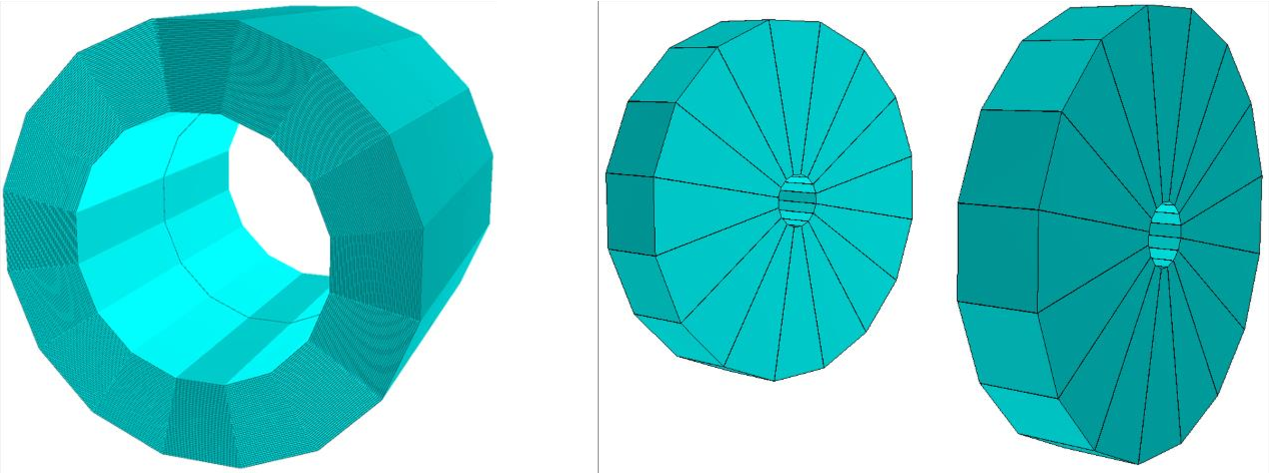
\includegraphics[width=0.9\textwidth]{Geometry.pdf}
\caption{Geometric configuration of the GS-HCAL system.
Left: barrel with 16~trapezoidal sectors forming a cylindrical structure
(inner diameter \SI{4280}{mm}, outer diameter \SI{6910}{mm}).
Right: endcap disks with matching sector segmentation.}
\label{fig:GS-geometry}
\end{figure}

The remainder of this paper is organised as follows.
Section~\ref{sec:design} describes the mechanical and geometrical design.
Sections~\ref{sec:gsdev}--\ref{sec:electronics} present the GS material
development, photon-detector characterisation, single-cell measurements,
calibration strategy, readout electronics, and prototype plans.
Section~\ref{sec:simperf} reports the full simulation and physics
performance.
Section~\ref{sec:alternatives} reviews alternative HCAL technologies,
and Section~\ref{sec:summary} summarises the results and outlines the
R\&D roadmap.

%% ====================================================================
\section{GS-HCAL design}
\label{sec:design}
%% ====================================================================

This section details the engineering implementation of the GS-HCAL\@.
The design translates the physics requirements into a modular mechanical
structure with 48~longitudinal layers, achieving a sampling fraction of
approximately 30\% while minimising the proportion of non-sensitive
material.
Each \SI{27.2}{mm}-thick layer combines \SI{9.8}{mm} steel absorbers
with \SI{10.2}{mm} GS active elements, maintaining a uniform cell
granularity of \cellsize throughout the barrel and endcap.

%% --------------------------------------------------------------------
\subsection{Single-layer structure}
\label{subsec:onelayer}
%% --------------------------------------------------------------------

The single-layer design of the GS-HCAL is illustrated in
Figure~\ref{fig:gshcal-cell}.
The calorimeter consists of alternating layers of GS cells (active
medium) and steel plates (absorber), providing high density with fine
segmentation for precise shower imaging.

Each layer has a total thickness of \SI{27.2}{mm}, corresponding to
approximately $0.125\,\lambdaI$.
From top to bottom the layer comprises:
a \SI{2}{mm} upper cover plate;
the \SI{10}{mm} GS active layer ($40\times40$~mm$^{2}$ cells);
a \SI{3.2}{mm} printed-circuit-board (PCB) layer carrying
application-specific integrated circuits (ASICs) for signal processing;
a \SI{2}{mm} bottom cover providing structural support; and
the \SI{9.8}{mm} steel absorber in which cooling pipes of \SI{3}{mm}
outer radius are embedded.
One SiPM is positioned at the centre of each GS cell on a PCB that
spans multiple cells.

The nuclear-interaction-length contributions of the steel absorber, GS,
and PCB are $0.0805\,\lambdaI$, $0.0425\,\lambdaI$, and
$0.0024\,\lambdaI$ (ratio $1:0.53:0.03$), respectively, yielding a
sampling fraction of approximately 31\%.

\begin{figure}[htbp]
\centering
\begin{subfigure}{0.50\linewidth}
  \centering
  \includegraphics[width=\linewidth]{GS-HCAL-cell.pdf}
  \caption{}
  \label{fig:gshcal-cell-a}
\end{subfigure}%
\begin{subfigure}{0.35\linewidth}
  \centering
  \includegraphics[width=\linewidth]{GSHCALOneCell1.pdf}
  \caption{}
  \label{fig:gshcal-cell-b}
\end{subfigure}
\caption{(a)~Single-layer structure of the GS-HCAL\@.
(b)~One GS cell of \cellsize.}
\label{fig:gshcal-cell}
\end{figure}

%% --------------------------------------------------------------------
\subsection{Barrel}
\label{subsec:barrel}
%% --------------------------------------------------------------------

The barrel is divided into 16~trapezoidal sectors
(Figure~\ref{fig:BarrelContourDimension}), with inner and outer radii
of \SI{2140}{mm} and \SI{3455}{mm} and a length of \SI{6460}{mm} along
the beam direction.
Each sector has a front width of \SI{851}{mm} and a back width of
\SI{1375}{mm}; its total thickness of \SI{1315}{mm} corresponds to
$6\,\lambdaI$.
The longitudinal segmentation into 48~layers follows the PFA
optimisation studies performed with the Plastic-Scintillator HCAL
(PS-HCAL) prototype~\cite{CALICE:2010fpb}.
The total barrel weight is \SI{955}{t}.

\begin{figure}[htbp]
\centering
\begin{subfigure}{0.42\linewidth}
  \centering
  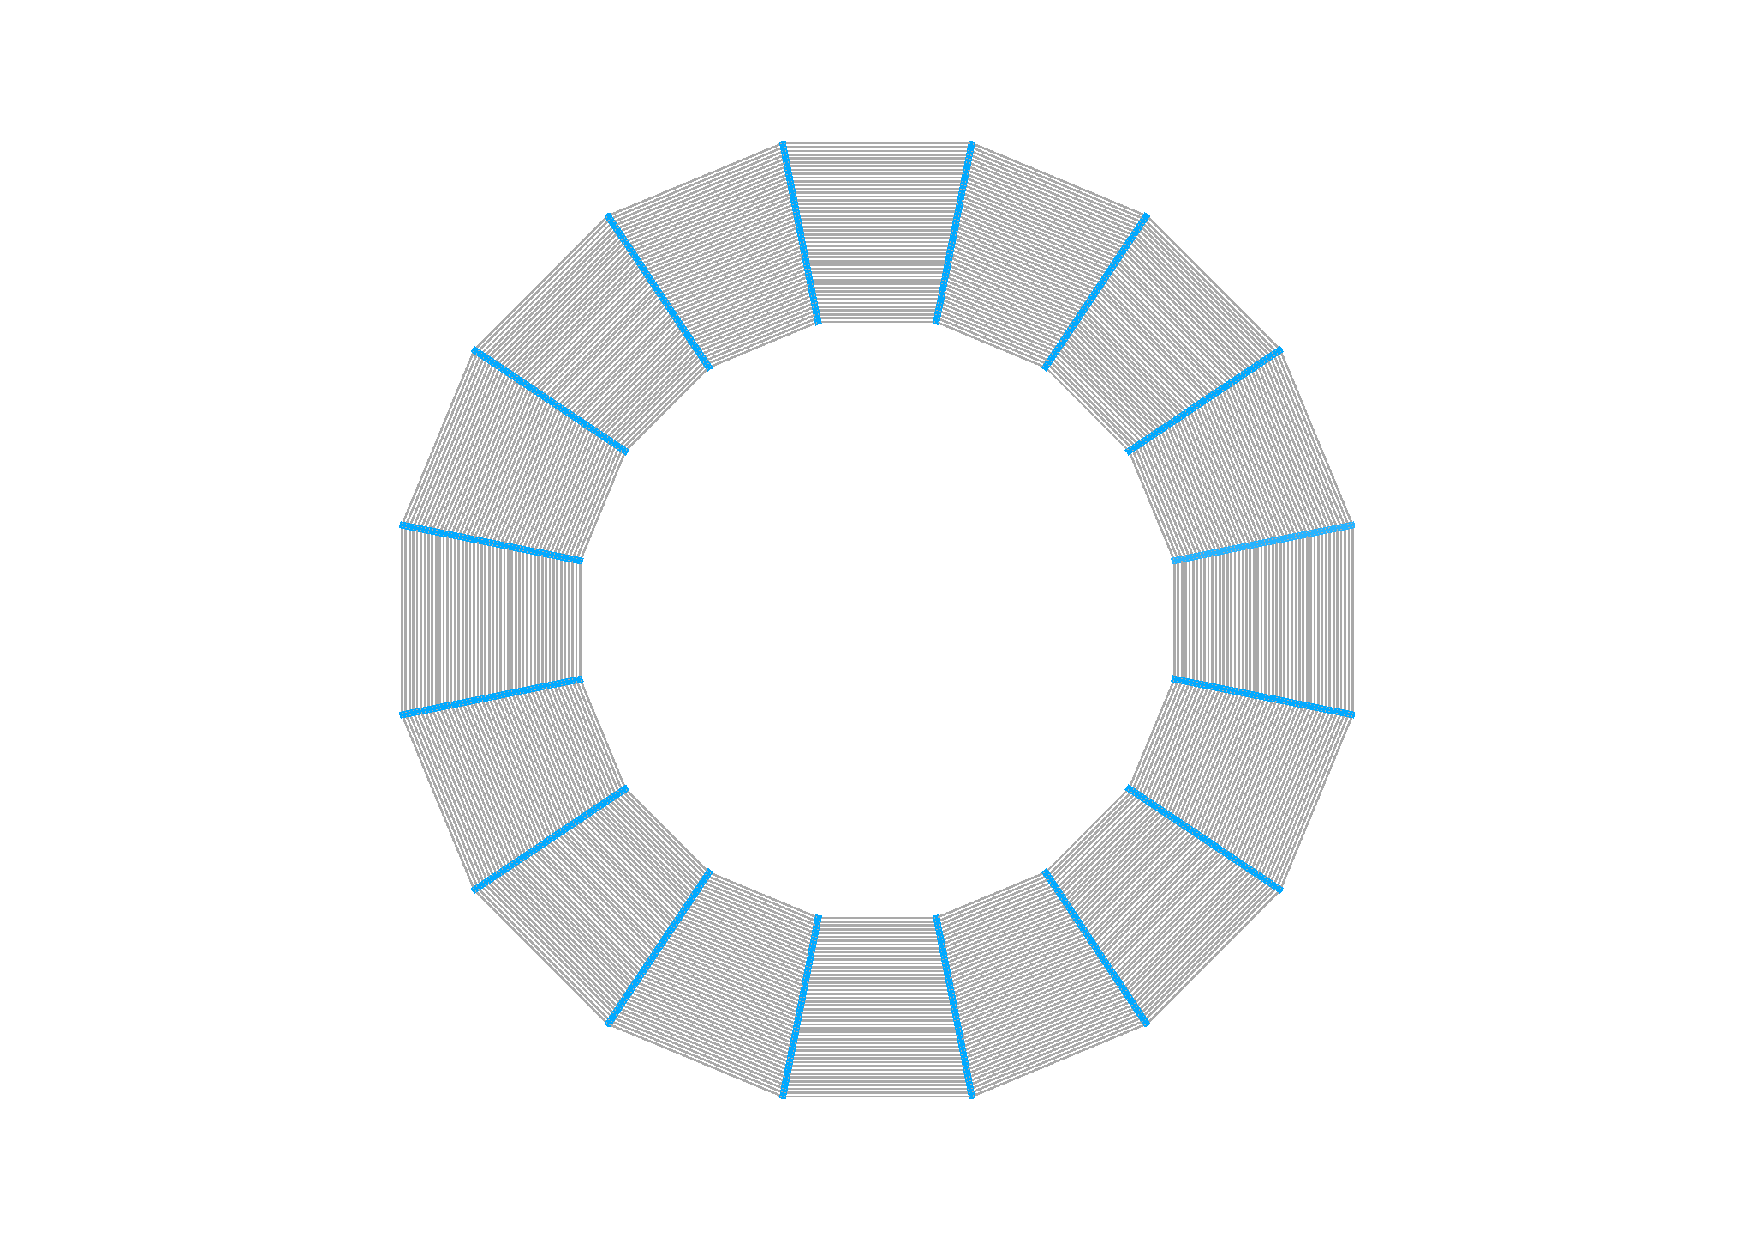
\includegraphics[width=\linewidth,trim=160pt 50pt 160pt 50pt,clip]{BarrelView1.pdf}
  \caption{}
\end{subfigure}\hfill
\begin{subfigure}{0.45\linewidth}
  \centering
  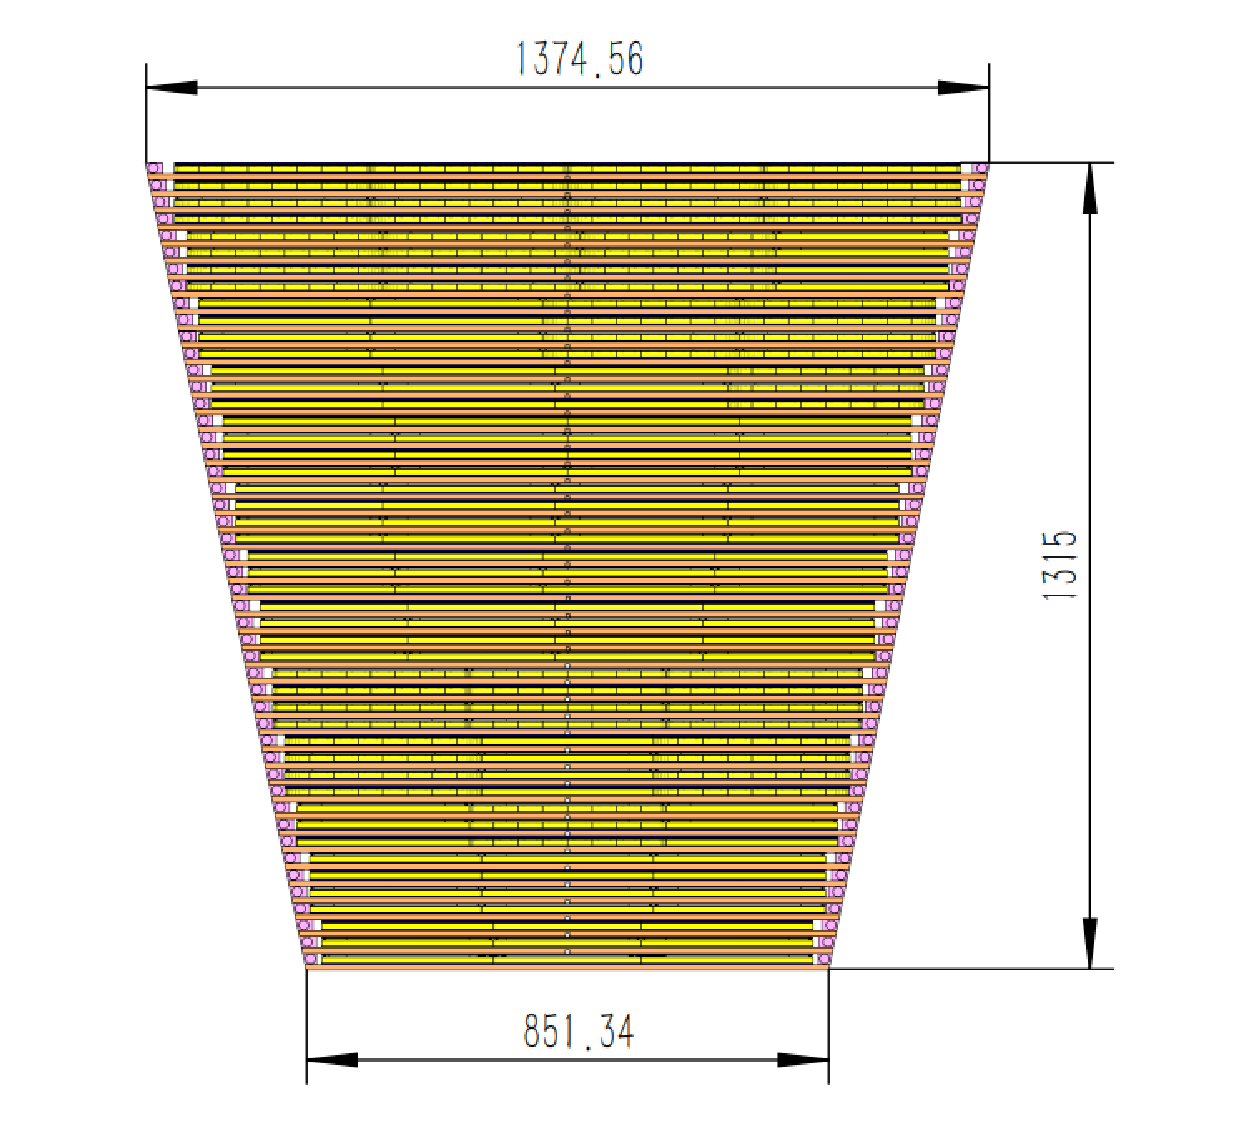
\includegraphics[width=\linewidth]{HCALBarrelOneSector.pdf}
  \caption{}
\end{subfigure}
\caption{Dimensions of the GS-HCAL barrel.
(a)~Cross-sectional view showing 16~trapezoidal sectors (inner diameter
\SI{4280}{mm}, outer diameter \SI{6910}{mm}).
(b)~Side view of a single trapezoidal sector (front width \SI{851}{mm},
back width \SI{1375}{mm}, depth \SI{1315}{mm}).}
\label{fig:BarrelContourDimension}
\end{figure}

The 16~radial sector boundaries introduce projective cracks, but
effective coverage is maintained through compensating mechanisms.
Hadronic showers predominantly initiate in the preceding BGO
electromagnetic calorimeter (ECAL), which provides $1.2\,\lambdaI$ of
upstream material and ensures lateral spread that bridges sector
boundaries.
The solenoidal magnetic field provides additional muon curvature away
from crack alignments.

Each layer consists of a steel absorber plate extending continuously
over the full \SI{6460}{mm} barrel length, upon which 30--40 modular
detection boxes are precisely positioned.
Each box contains a complete detection unit: GS cells, SiPMs, PCB, ASIC
chips, cables, and cover plates.
Taking the 48th (outermost) layer as an example
(Figure~\ref{fig:M-1}), 40~boxes are arranged in 4~rows along $\phi$
with 10~boxes per row, each containing $8\times16=128$ cells and giving
5120~cells per layer.
Each box is aligned with registration pins and secured with four corner
bolts; a \SI{2}{mm} gap between adjacent boxes accommodates thermal
expansion.

\begin{figure}[htbp]
\centering
\includegraphics[width=0.7\linewidth]{BarrelSectorWithLayer.pdf}
\caption{A barrel sector of the GS-HCAL, showing the arrangement of
40~boxes in the outermost (48th) layer.
The four quadrants~(1)--(4) each contain 10~boxes numbered $n$-1 to
$n$-10.}
\label{fig:M-1}
\end{figure}

The trapezoidal geometry requires adaptive box arrangements across the
48~layers.  Three box widths (\SI{320}{mm}, \SI{280}{mm}, and
\SI{240}{mm}) are combined to maintain full coverage while preserving
the \cellsize cell granularity (Figure~\ref{fig:BarrelModuleStructure}).

\begin{figure}[htbp]
\centering
\includegraphics[width=0.9\linewidth]{Fig.1.81-Boxes_dimension-and_more-structure_details.pdf}
\caption{GS-HCAL barrel sector structure.
Left~(a): full sector composed of 48~layers.
Centre~(b): dimensions of an individual box
(widths 240/280/\SI{320}{mm}, length \SI{646}{mm}).
Right~(c): internal structure of a single box, including cover plates,
GS~cells, PCB with ASICs, cables, and cooling-water pipes.}
\label{fig:BarrelModuleStructure}
\end{figure}

A water-cooling system manages the thermal load of the front-end ASICs
(\SI{15}{mW} per channel).
For the 48th layer the heat load is \SI{76.8}{W}
($5120\text{ ch}\times\SI{15}{mW/ch}$).
Each of the 48~layers in a sector incorporates four water-cooling pipes
embedded in the steel absorber.
Every eight consecutive layers share common input and output manifolds
(Figure~\ref{fig:BarrelCooling}), resulting in six independent cooling
loops per sector.
Round pipes of \SI{3}{mm} outer radius are used.

\begin{figure}[htbp]
\centering
\begin{subfigure}{0.55\linewidth}
  \centering
  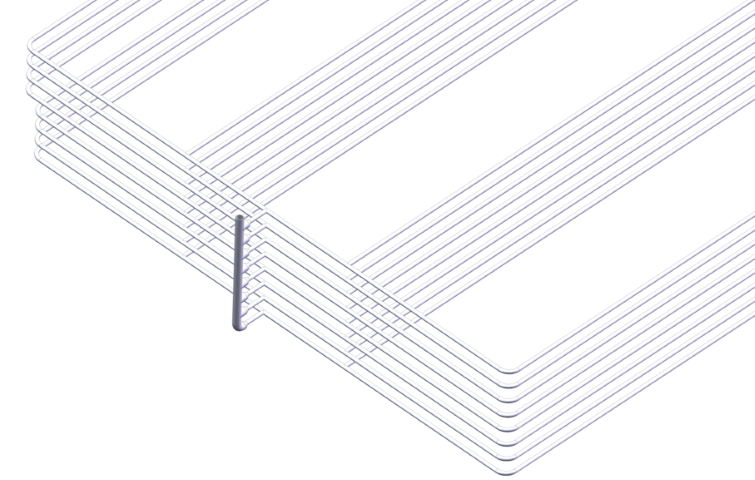
\includegraphics[width=\linewidth]{CoolingBarrelLeft.png}
  \caption{}
\end{subfigure}\hfill
\begin{subfigure}{0.35\linewidth}
  \centering
  \includegraphics[width=\linewidth]{CoolingBarrelv2.jpg}
  \caption{}
\end{subfigure}
\caption{Cooling-pipe routing for a barrel sector.
(a)~Schematic of the eight-in-one pipeline design.
(b)~Simulated coolant flow-velocity distribution (m/s), with inlet and
outlet positions indicated.}
\label{fig:BarrelCooling}
\end{figure}

The barrel component weights are summarised in
Table~\ref{tab:BarrelWeight}.

\begin{table}[htbp]
\centering
\caption{Weight breakdown of the barrel GS-HCAL\@.}
\label{tab:BarrelWeight}
\begin{tabular}{l S[table-format=5.0] S[table-format=3.1]}
\toprule
\textbf{Component} & {\textbf{Weight/sector (kg)}} & {\textbf{Weight/barrel (t)}} \\
\midrule
Cover plate        & 10287 & 164.6 \\
PCB plate          &   390 &   6.2 \\
Glass scintillator & 19277 & 308.4 \\
Absorber layer     & 27515 & 440.2 \\
Support structure  &  1883 &  30.1 \\
Auxiliaries        &   350 &   5.6 \\
\midrule
Total              & 59702 & 955.2 \\
\bottomrule
\end{tabular}
\end{table}

%% --------------------------------------------------------------------
\subsection{Endcap}
\label{subsec:endcap}
%% --------------------------------------------------------------------

The two endcaps complement the barrel to provide full geometric coverage
along the beam direction.
Each endcap disk (Figure~\ref{fig:EndcapsOverall}) matches the barrel
design with 16~sectors, inner and outer radii of \SI{450}{mm} and
\SI{3455}{mm}, and a total thickness of \SI{1315}{mm} divided among
48~layers.
A single sector has a top width of \SI{1307}{mm} and a radial height of
\SI{2862}{mm}, and is divided into 6~boxes along the radial direction.
Each endcap weighs \SI{362}{t}.

\begin{figure}[htbp]
\centering
\begin{subfigure}{0.58\linewidth}
  \centering
  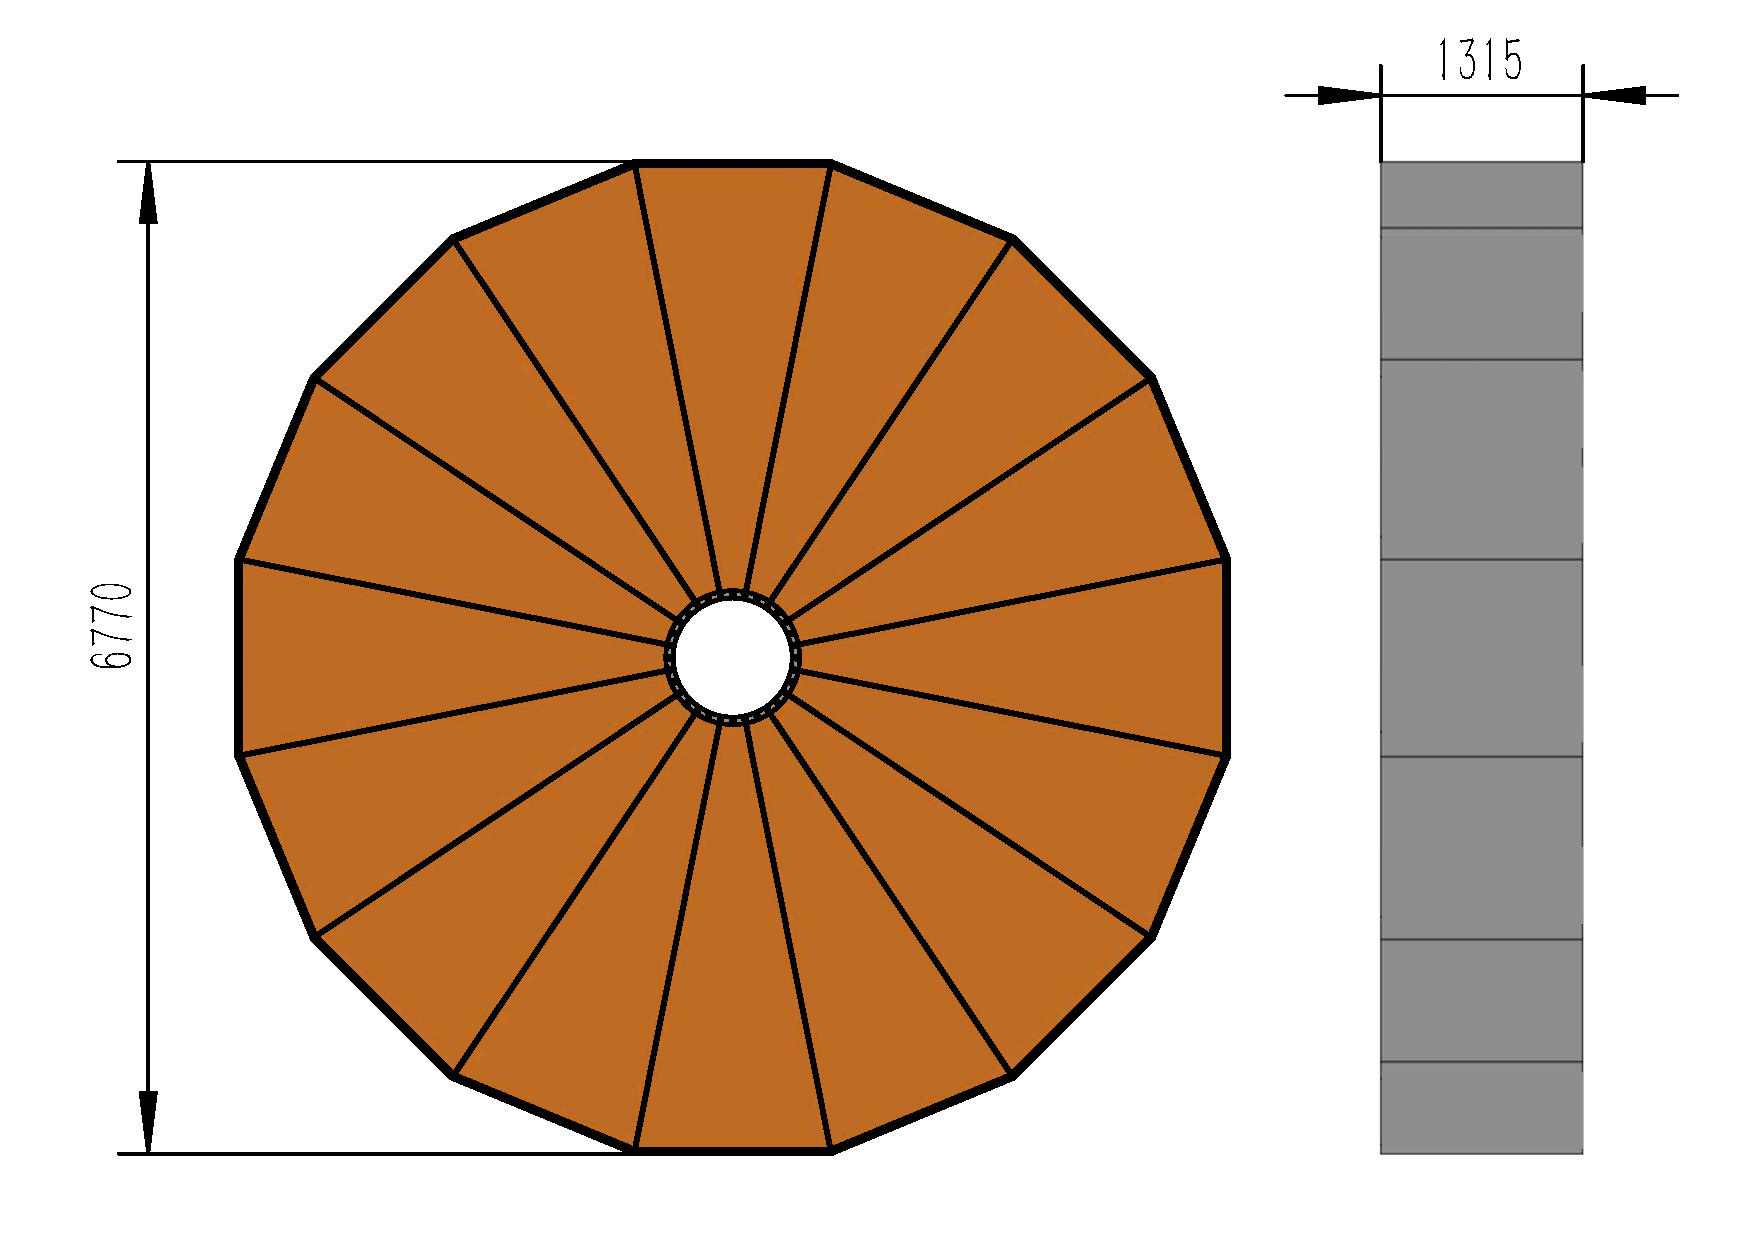
\includegraphics[width=\linewidth]{HCALEndcapOverall.pdf}
  \caption{}
\end{subfigure}\hfill
\begin{subfigure}{0.20\linewidth}
  \centering
  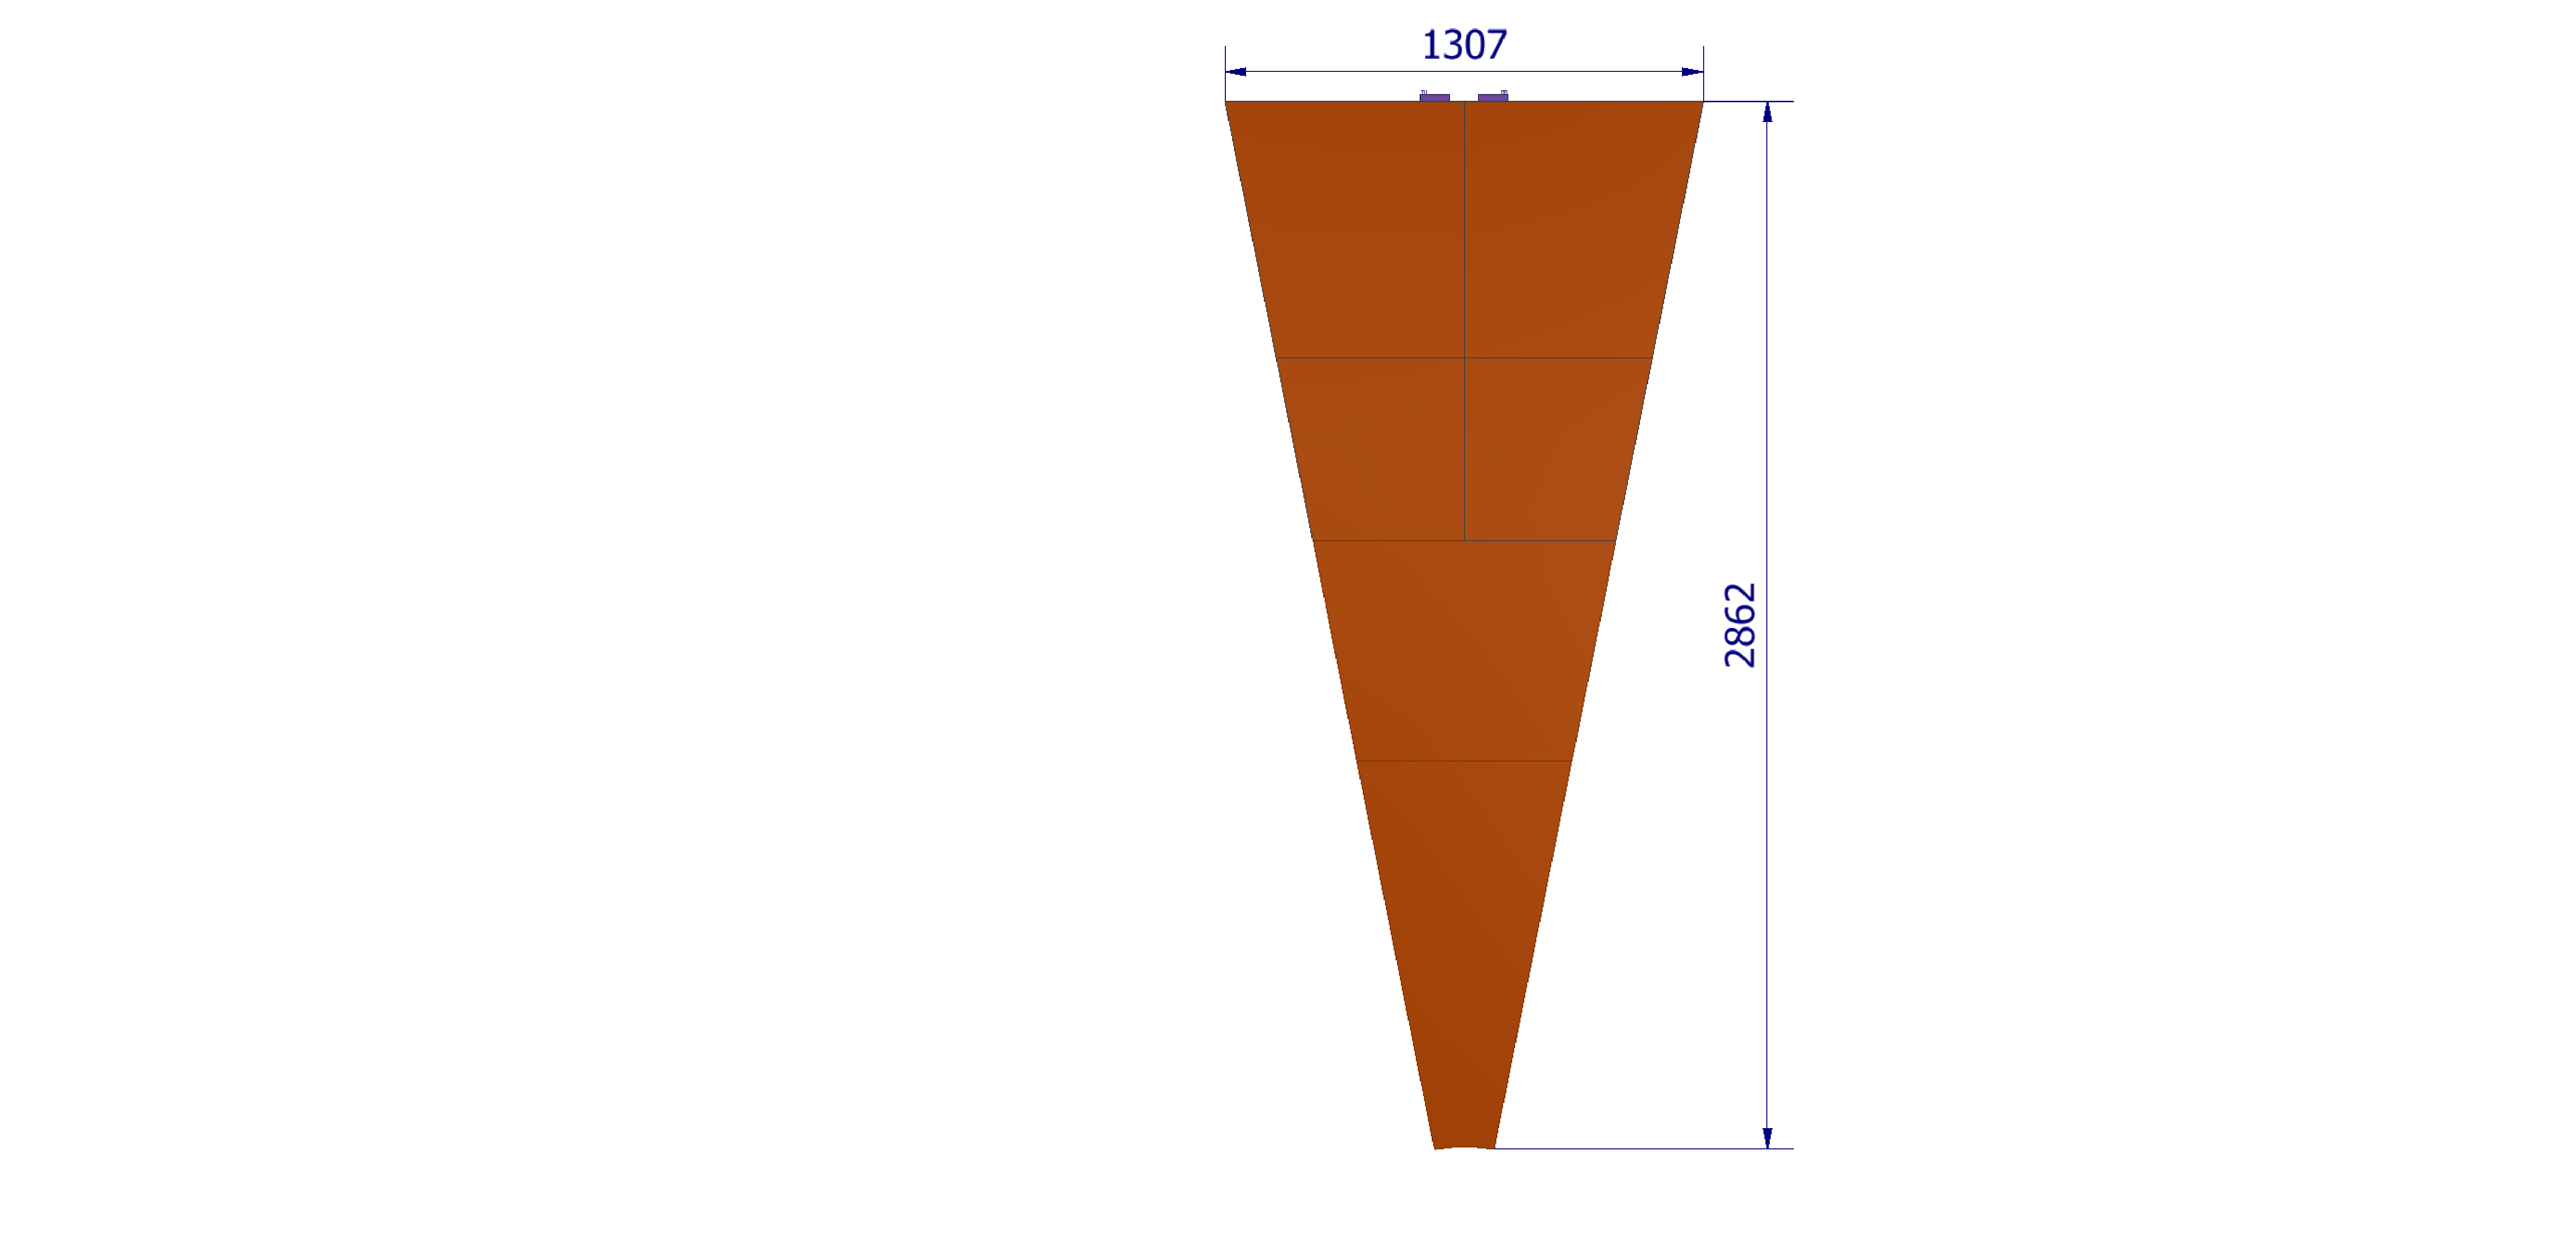
\includegraphics[width=\linewidth]{HCALEndcapOneSector.pdf}
  \caption{}
\end{subfigure}
\caption{Dimensions of the GS-HCAL endcaps.
(a)~Front and side views (full diameter \SI{6670}{mm}, thickness
\SI{1315}{mm}).
(b)~Single sector; the complete endcap comprises 16~such sectors.}
\label{fig:EndcapsOverall}
\end{figure}

Construction begins with 1405~detector cells assembled into one sector
layer; 16~sector layers form a complete disk-shaped layer, and
48~layers are stacked to complete the module.
A \SI{50}{mm}-thick outer structural plate provides rigidity and serves
as the installation reference.
Active layers and steel absorber plates are alternately installed
horizontally and then rotated into the final vertical orientation.

The endcap cooling system provides 16~separate cooling regions per layer
(Figure~\ref{fig:M-14}), each with one dedicated water channel.
When all 48~layers are assembled the matching channels connect vertically,
forming 48~parallel water circuits with \SI{12}{mm} inner-diameter pipes.

\begin{figure}[htbp]
\centering
\begin{subfigure}{0.50\linewidth}
  \centering
  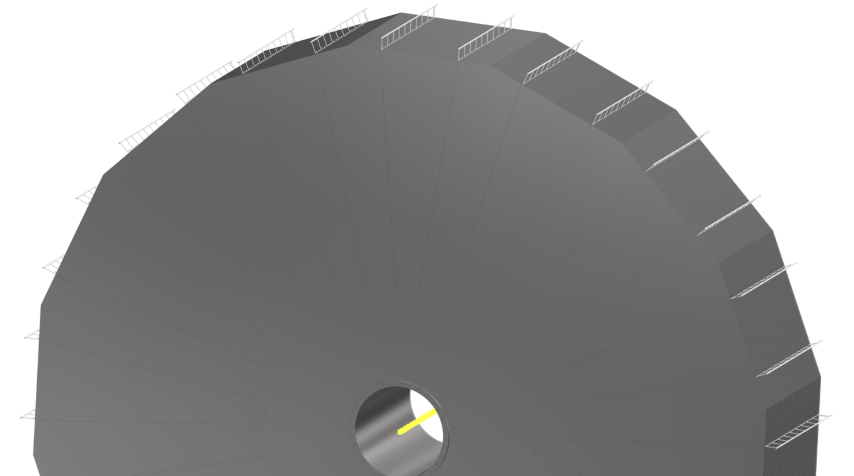
\includegraphics[width=\linewidth]{CoolingEndcapHalf.png}
  \caption{}
\end{subfigure}\hfill
\begin{subfigure}{0.42\linewidth}
  \centering
  \raisebox{0.1cm}{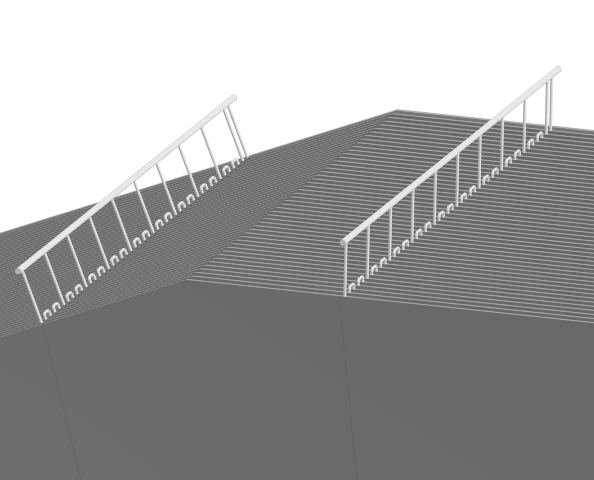
\includegraphics[width=\linewidth]{CoolingEndcapPart.png}}
  \caption{}
\end{subfigure}
\caption{Endcap cooling-pipe structure: (a)~half of the endcap;
(b)~zoomed corner view.}
\label{fig:M-14}
\end{figure}

%% --------------------------------------------------------------------
\subsection{Mechanical feasibility}
\label{subsec:mechanics}
%% --------------------------------------------------------------------

Structural finite-element analysis validates the mechanical feasibility
of the GS-HCAL design.
Particular attention was paid to the barrel's capacity to support the
\SI{135}{t} ECAL while preserving alignment precision.
Figure~\ref{fig:deformation_barrel} shows the deformation distribution
with and without ECAL loading.

\begin{figure}[htbp]
\centering
\begin{subfigure}{0.80\linewidth}
  \centering
  \includegraphics[width=\linewidth]{1.7.1.3.3-3.png}
  \caption{}
\end{subfigure}

\vspace{0.3cm}

\begin{subfigure}{0.80\linewidth}
  \centering
  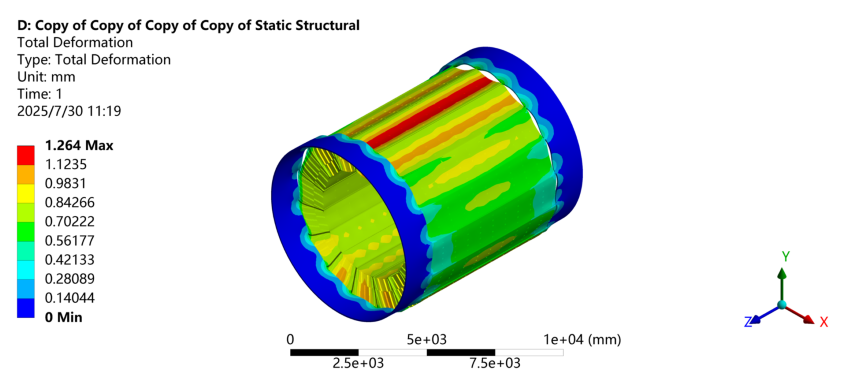
\includegraphics[width=\linewidth]{1.7.1.3.3-2.png}
  \caption{}
\end{subfigure}
\caption{Deformation distribution of the GS-HCAL (a)~without and
(b)~with ECAL loading.}
\label{fig:deformation_barrel}
\end{figure}

During assembly maximum deformations remain below \SI{0.66}{mm} with
localised stresses of \SI{190}{MPa}, well below the yield strength of
the structural materials.
Under the full ECAL load, peak stresses reach \SI{371}{MPa} at specific
connection points; these critical areas employ titanium-alloy (TC4)
components maintaining safety factors above~2.2, while the bulk of the
structure uses standard stainless steel.
Layer-to-layer deformation differences remain below \SI{0.2}{mm}
(within the \SI{2.4}{mm} gasket accommodation range), and intra-layer
deformations are constrained to less than \SI{0.5}{mm}, producing only
\SI{20}{MPa} stress in the GS cells.
The scintillator boxes withstand \SI{0.5}{mm} bending with a safety
factor exceeding three.

%% --------------------------------------------------------------------
\subsection{Channel count summary}
\label{subsec:summary_design}
%% --------------------------------------------------------------------

Table~\ref{tab:GSHCALQuantities} summarises the cell, box, layer, and
sector counts.
The complete detector contains approximately 5.22~million readout
channels.

\begin{table}[htbp]
\centering
\caption{Numbers of cells, boxes, layers, and sectors for the barrel and
endcap.}
\label{tab:GSHCALQuantities}
\begin{tabular}{lcccc}
\toprule
\textbf{Part} & \textbf{Cells} & \textbf{Boxes} & \textbf{Layers} &
\textbf{Sectors} \\
\midrule
Barrel             & 3\,212\,800          & 27\,840        & $48\times16$
& 16 \\
Endcap ($\times2$) & $1\,006\,080\times2$ & $3072\times2$  &
$48\times16\times2$ & $16\times2$ \\
\bottomrule
\end{tabular}
\end{table}

%% ====================================================================
\section{Glass-scintillator development}
\label{sec:gsdev}
%% ====================================================================

%% --------------------------------------------------------------------
\subsection{Historical context}
\label{subsec:history}
%% --------------------------------------------------------------------

The use of glass scintillators (GS) in calorimetry dates back to the
1980s, when the Crystal Clear Collaboration at
CERN~\cite{Buchner:1988fu} pioneered investigations into high-$Z$ glass
matrices for electromagnetic calorimeters.
The HED-1 GS prototype~\cite{Buchner:1988fu} demonstrated the
material's potential but was limited by short radiation length and low
light output; subsequent work on cerium-doped heavy-flint glass
(HFG:Ce) revealed insufficient radiation hardness for high-luminosity
environments.
A persistent limitation of traditional GS was excessive self-absorption,
which severely attenuated the light output in long-bar geometries and
stifled numerous design proposals.

The maturation of SiPM technology and the adoption of PFA-based
calorimetry in the 2010s fundamentally changed the
picture~\cite{Tang:2022yrb,Hu:2023dbm,Hu:2024nvo}.
Mass-produced SiPMs drastically reduced the cost of high-efficiency
photodetection, while PFA granular segmentation eliminated the need for
long light-transmission paths by employing compact, optically isolated
cells.
These innovations relaxed the light-yield requirements to a minimum of
approximately \SI{1000}{\phMeV}, provided the SiPMs exhibit a photon
detection efficiency (PDE) of $\geq40\%$.

Post-2020 advances initiated by the Institute of High Energy Physics
(IHEP)~\cite{LAN2022113000,YU2023113846,ZHU2024} focused on optimising
the density--light-yield balance while ensuring manufacturing
scalability.
The GS-HCAL initiative, benefiting from the PS-HCAL design of the
CALICE Collaboration~\cite{calice,CALICE:2010fpb}, employs GS cells
with densities of approximately \SI{6}{g/cm^{3}} read out by SiPM
arrays.

%% --------------------------------------------------------------------
\subsection{GFO glass: material properties}
\label{subsec:gfo}
%% --------------------------------------------------------------------

Over the past seven years the Glass-Scintillator Collaboration, led by
IHEP and comprising universities, research institutes, and industrial
partners, has systematically developed various glass
compositions~\cite{LAN2022113000,YU2023113846,ZHU2024}.
Figure~\ref{fig:GSGroup} shows the light yield versus density for the
GS samples investigated.

\begin{figure}[htbp]
\centering
\includegraphics[width=0.7\textwidth]{GSGroup.pdf}
\caption{Light yield versus density for GS samples developed by the
Glass-Scintillator Collaboration and other groups.}
\label{fig:GSGroup}
\end{figure}

Gadolinium fluoro-oxide (GFO) glass was selected as the baseline
material for its optimal balance between performance and
manufacturability~\cite{HUA202523367,Hua:2023myf,Hua:2024djh}.
Table~\ref{tab:GS1} compares its key parameters with those of BGO
crystal~\cite{BGO} and DSB glass~\cite{Dormenev:2021vtn}.
GFO achieves a density of \SI{6.0}{g/cm^{3}} with a radiation length of
\SI{1.59}{cm} and a nuclear interaction length of \SI{24.2}{cm}.
The composition features Ce$^{3+}$ as the luminescent centre, chosen for
its strong emission, fast decay, and efficient energy transfer from
Gd$^{3+}$ modifiers~\cite{GS-1}.
The borosilicate matrix (B$_{2}$O$_{3}$--SiO$_{2}$) provides excellent
thermal and optical stability, with Al$_{2}$O$_{3}$ additives enhancing
chemical durability.
Gadolinium serves as the heavy-element modifier, offering high density,
low intrinsic radioactivity, and cost-effectiveness compared with
lanthanum or lutetium alternatives.

\begin{table}[htbp]
\centering
\caption{Key parameters of GFO glass ($5\times5\times5$~mm$^{3}$ sample)
compared with BGO crystal~\cite{BGO} and DSB
glass~\cite{Dormenev:2021vtn}.}
\label{tab:GS1}
\begin{tabular}{lccc}
\toprule
\textbf{Parameter} & \textbf{GFO} & \textbf{BGO} & \textbf{DSB} \\
\midrule
Density (g/cm$^{3}$)                       & 6.0      & 7.13  & 4.2   \\
Melting point ($^{\circ}$C)                 & 1250     & 1050  & 1550  \\
Radiation length (cm)                       & 1.59     & 1.12  & 2.62  \\
Moli\`{e}re radius (cm)                    & 2.49     & 2.23  & 3.33  \\
Nuclear interaction length (cm)             & 24.2     & 22.7  & 31.8  \\
$Z_{\mathrm{eff}}$                          & 56.6     & 71.5  & 49.7  \\
$dE/dx$ (MeV/cm)                            & 8.0      & 8.99  & 5.9   \\
Emission peak (nm)                          & 400      & 480   & 430   \\
Refractive index                            & 1.74     & 2.15  & ---   \\
Light yield (ph/MeV)                        & ${\sim}1500$ & 7500  & 2500  \\
Energy resolution (\% at \SI{662}{keV})     & ${\sim}23$   & 9.5   & ---   \\
Scintillation decay time (ns)               & ${\sim}60$, 500 & 60, 300 & 90, 400 \\
\bottomrule
\end{tabular}
\end{table}

%% --------------------------------------------------------------------
\subsection{Light yield}
\label{subsec:lightyield}
%% --------------------------------------------------------------------

Figure~\ref{fig:LargeGS} shows GFO glass cells of \cellsize under
natural and ultraviolet light.
Figure~\ref{fig:GS40}(a) presents the X-ray-excited luminescence (XEL)
and optical-transmission spectra; the transmittance in the visible range
exceeds 80\%, with a self-absorption effect
observed~\cite{SUI2025100878} near the \SI{400}{nm} emission peak.
Extensive $\gamma$-ray testing confirms that the GFO light yield
consistently exceeds \SI{1000}{\phMeV}.
When measured with an XP2020 (\SI{2}{inch}) photomultiplier tube (PMT),
the detected photoelectron number reaches one-third that of BGO crystals
of identical dimensions~\cite{GS-5}
(Figure~\ref{fig:GS40}b).
Figure~\ref{fig:GS40}(c) shows the scintillation decay profile under
$\gamma$-ray excitation: the slow-component decay time is controlled
below \SI{500}{ns}, which is fully compatible with the high granularity
of the GS-HCAL design.

\begin{figure}[htbp]
\centering
\begin{subfigure}{0.40\textwidth}
  \centering
  \includegraphics[width=\linewidth]{GSN.pdf}
  \caption{}
\end{subfigure}\hfill
\begin{subfigure}{0.42\textwidth}
  \centering
  \includegraphics[width=\linewidth]{GSUV.pdf}
  \caption{}
\end{subfigure}
\caption{GFO glass cells (\cellsize) under (a)~natural light and
(b)~ultraviolet illumination.}
\label{fig:LargeGS}
\end{figure}

\begin{figure}[htbp]
\centering
\begin{subfigure}{0.50\textwidth}
  \centering
  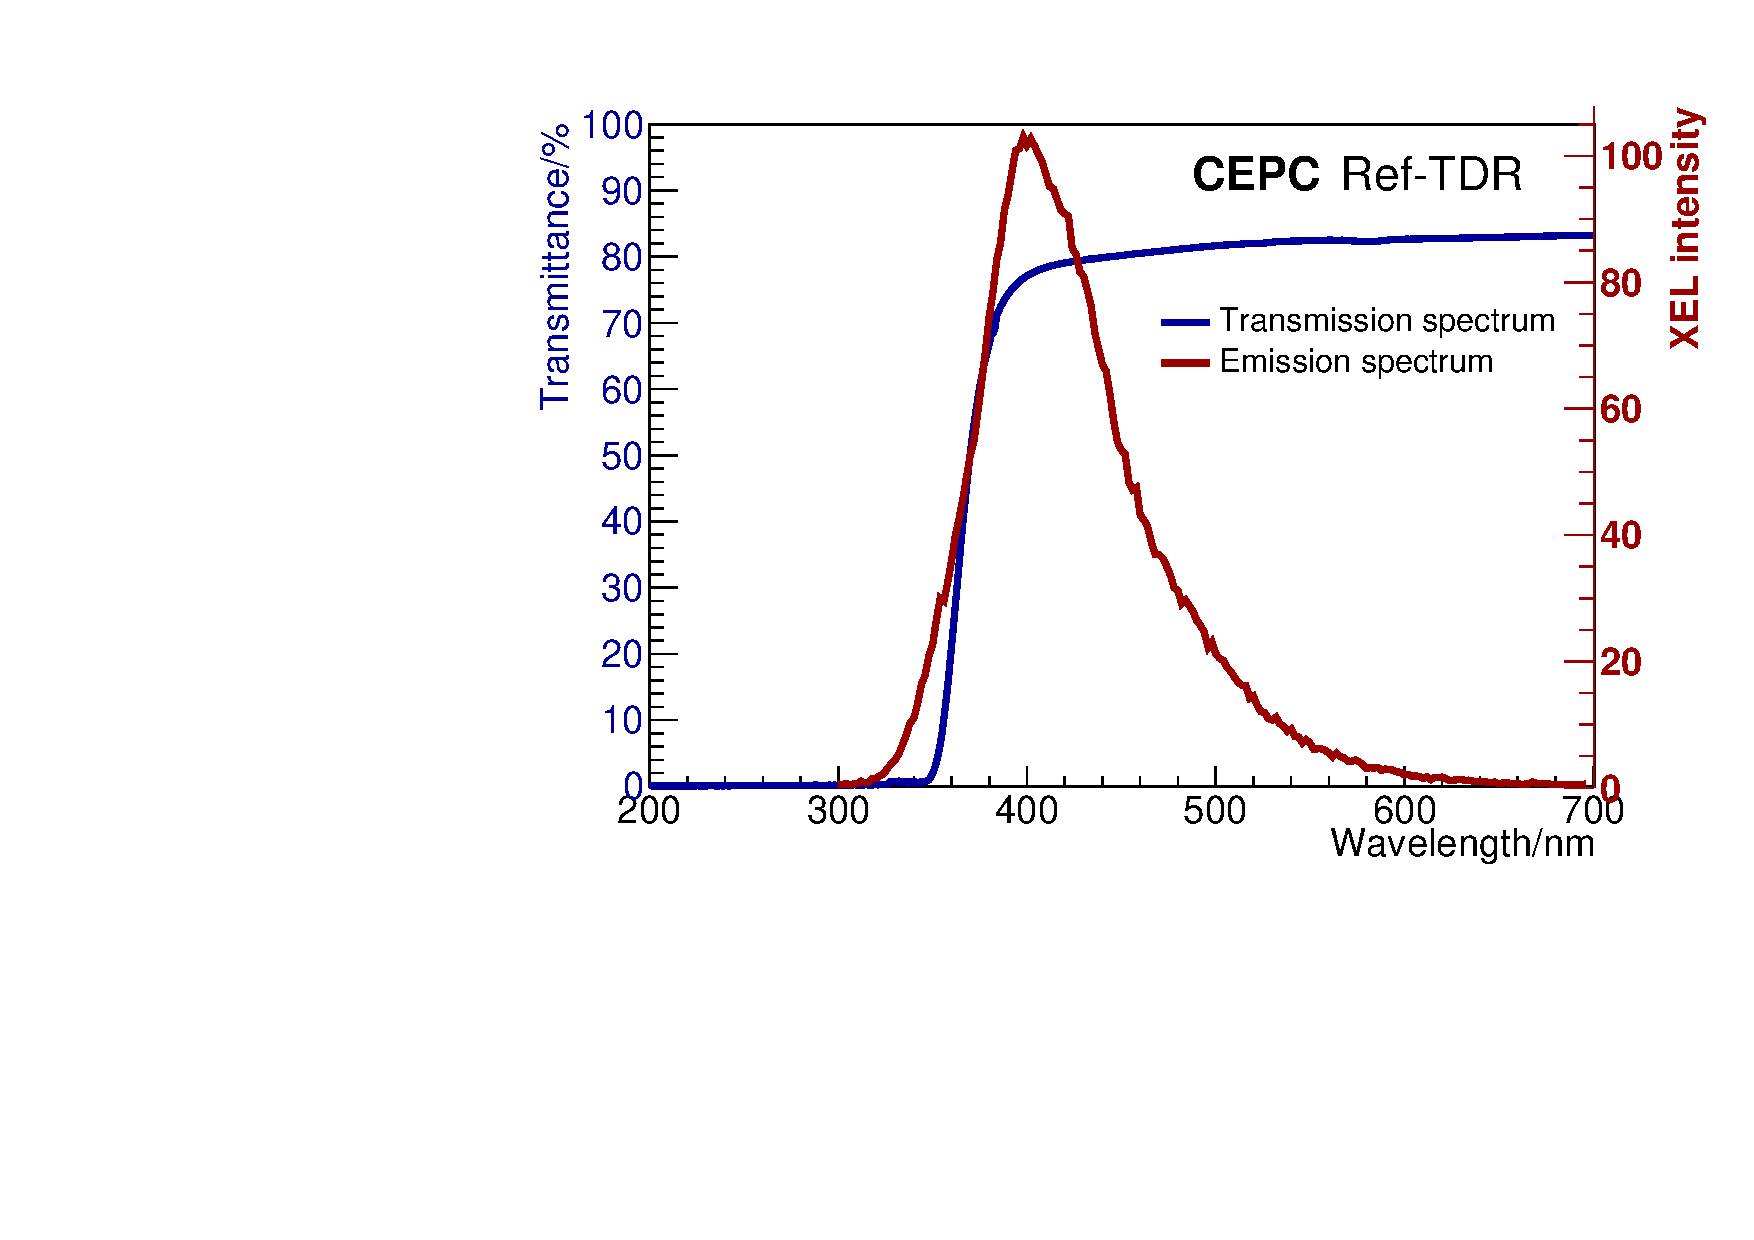
\includegraphics[width=\linewidth]{newGS40-A.pdf}
  \caption{}
  \label{fig:GS40-a}
\end{subfigure}

\vspace{0.3cm}

\begin{subfigure}{0.45\textwidth}
  \centering
  \includegraphics[width=\linewidth]{GS40-b.pdf}
  \caption{}
  \label{fig:GS40-b}
\end{subfigure}\hfill
\begin{subfigure}{0.45\textwidth}
  \centering
  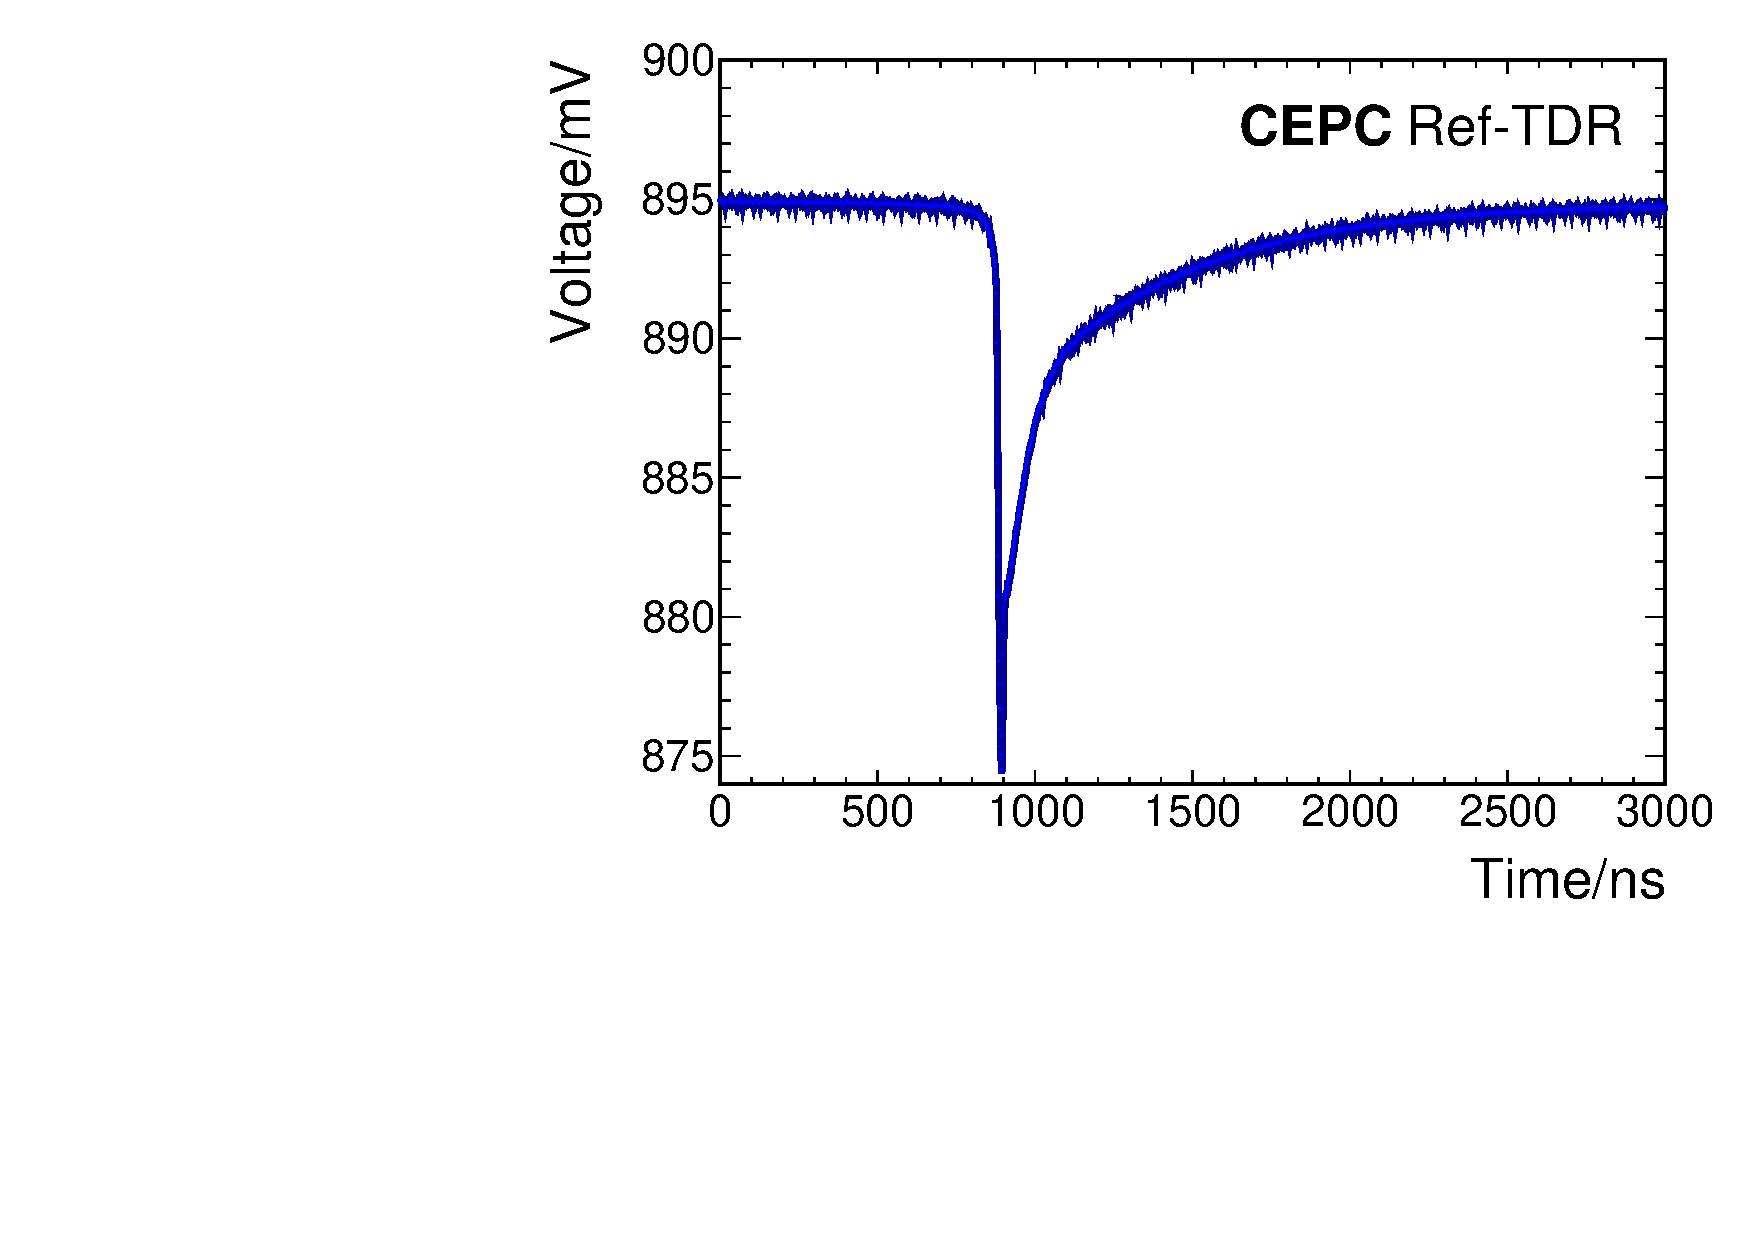
\includegraphics[width=\linewidth]{GS40-c.pdf}
  \caption{}
  \label{fig:GS40-c}
\end{subfigure}
\caption{(a)~Optical-transmission and XEL spectra of the GFO glass.
(b)~Energy spectra of GFO GS and BGO crystal of the same dimensions.
(c)~Scintillation decay curve of the GFO glass.}
\label{fig:GS40}
\end{figure}

%% --------------------------------------------------------------------
\subsection{Light attenuation length}
\label{subsec:attenuation}
%% --------------------------------------------------------------------

The light attenuation length (LAL, $L_{0}$) is determined through
thickness-dependent transmittance measurements using~\cite{Zhu:1996tt}
\begin{equation}
\label{eq:LAL}
L_{0} = \frac{L_{2}-L_{1}}{\ln(T_{L_{1}}/T_{L_{2}})},
\end{equation}
where $L_{1}$ and $L_{2}$ ($L_{2}>L_{1}$) denote two sample
thicknesses and $T_{L_{i}}$ the corresponding transmittance values.

As shown in Figure~\ref{fig:newLAL1}, the best-performing GFO sample
achieves $L_{0}\approx\SI{6}{cm}$ at \SI{400}{nm} (the GS emission
peak).
Across the visible spectrum above \SI{400}{nm} the LAL remains stable
between \SI{6}{cm} and \SI{6.8}{cm}.

\begin{figure}[htbp]
\centering
\includegraphics[width=0.60\textwidth]{NewLAL1.pdf}
\caption{Attenuation length of GFO glass versus wavelength, measured
using the transmittance method.}
\label{fig:newLAL1}
\end{figure}

%% --------------------------------------------------------------------
\subsection{Radiation tolerance}
\label{subsec:radiation}
%% --------------------------------------------------------------------

Under the current CEPC operating plan the accumulated radiation dose
reaches \SI{40}{Gy} during the 10-year Higgs run (luminosity
$\mathcal{L}=8\times10^{34}$~cm$^{-2}$s$^{-1}$).
For the $Z$-pole run ($\mathcal{L}=192\times10^{34}$~cm$^{-2}$s$^{-1}$),
one year of operation yields an estimated dose of approximately
\SI{96}{Gy}.
As shown in Figure~\ref{fig:gamma-irradiation}, the GFO light yield
retains more than 70\% of its initial value for doses below
\SI{100}{Gy}.
This result is confirmed by proton-beam irradiation
tests~\cite{YIN2026170869} at the APEP
facility~\cite{Liu:2022czi}.

\begin{figure}[htbp]
\centering
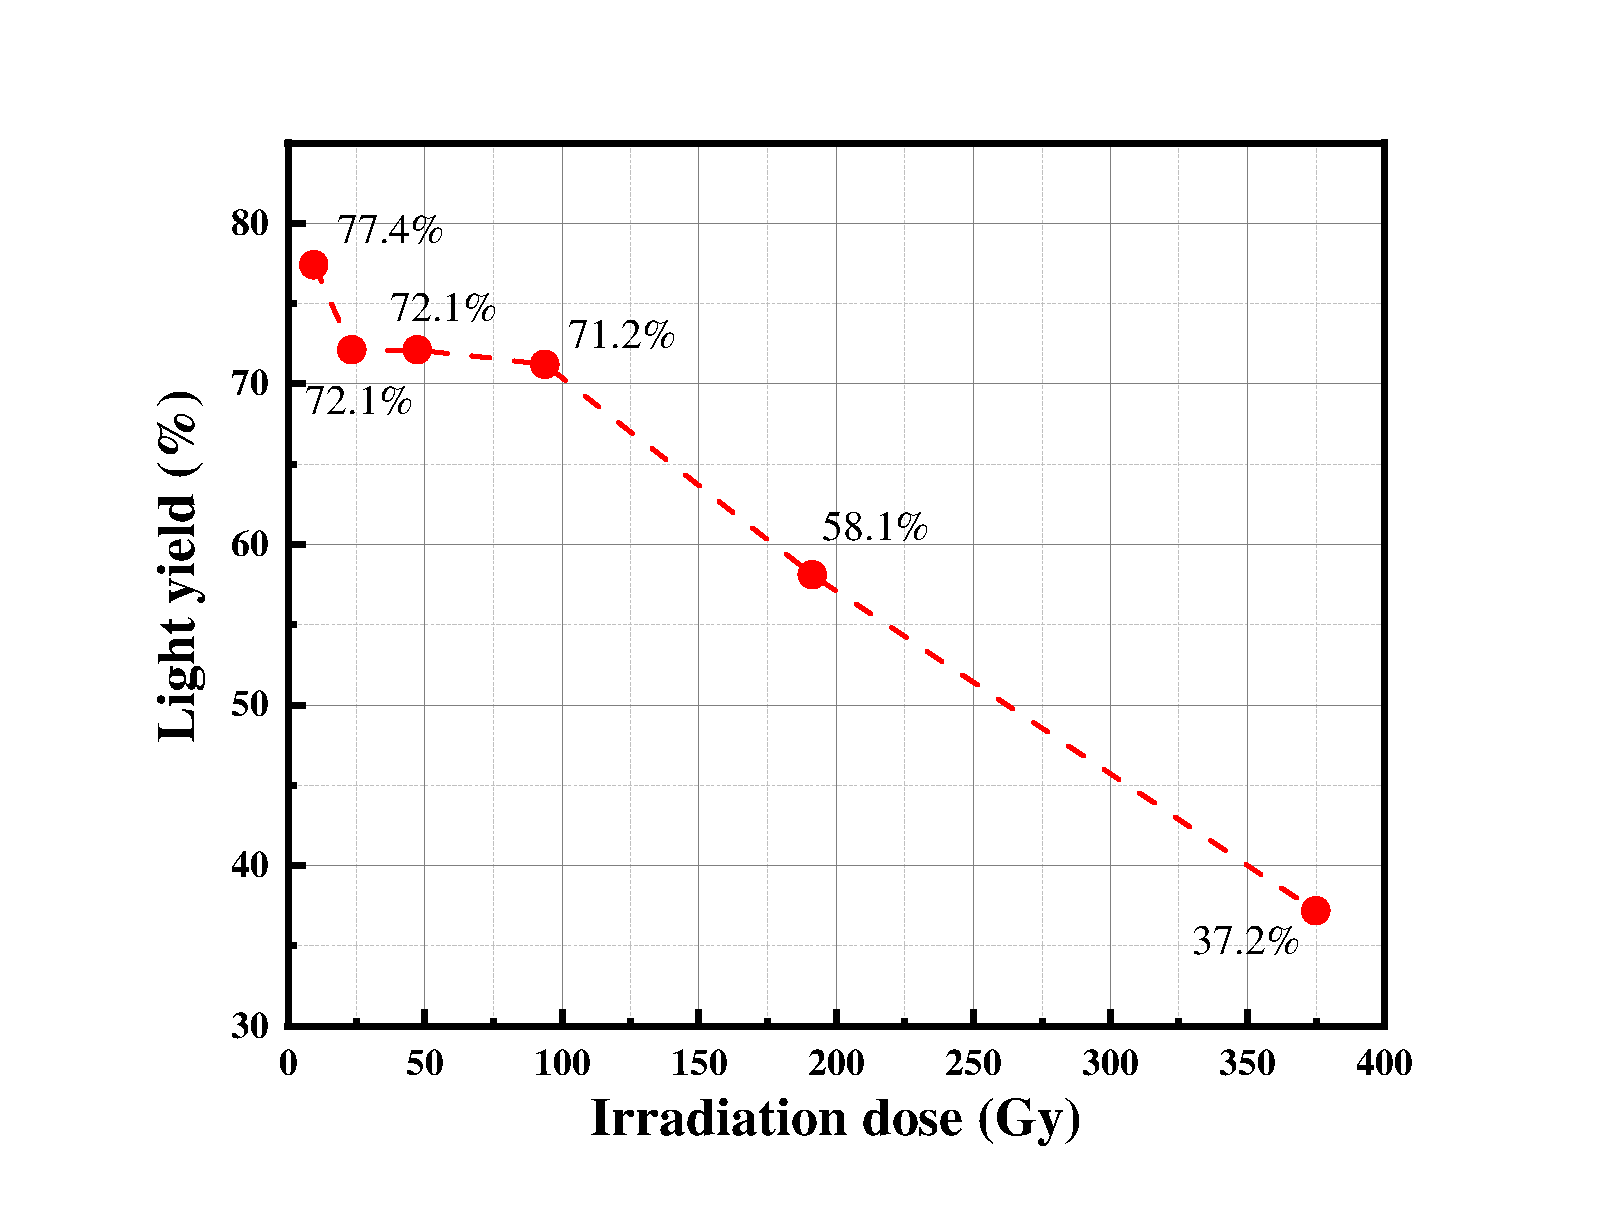
\includegraphics[width=0.60\linewidth]{LightYieldReductionGammaIrradiation.pdf}
\caption{Relative light yield of GFO glass as a function of
$\gamma$-irradiation dose.  At \SI{100}{Gy} the retention is 71.2\%.}
\label{fig:gamma-irradiation}
\end{figure}

%% --------------------------------------------------------------------
\subsection{Quality control}
\label{subsec:qc}
%% --------------------------------------------------------------------

Reproducible GS tile production with controlled quality is essential for
the technology validation.
Approximately 290~tiles of \cellsize have been produced to date; about
60\% meet the target light yield exceeding \SI{1000}{\phMeV}.
Tile-to-tile light-yield variations will be corrected through dedicated
calibration, including a light-emitting-diode (LED) monitoring system
and minimum-ionising-particle (MIP) inter-calibration using muon beams
or cosmic rays.

A production run of approximately 10\,000~tiles is scheduled for
2025--2026 to equip the full-size prototype.
An automated batch-testing platform is being developed to measure tile
properties rapidly and to enforce rigorous quality-control metrics:
light-yield uniformity, attenuation-length verification, and
dimensional tolerances.

%% ====================================================================
\section{Photon detector and optical simulation}
\label{sec:photondet}
%% ====================================================================

%% --------------------------------------------------------------------
\subsection{SiPM selection and characterisation}
\label{subsec:sipm}
%% --------------------------------------------------------------------

Silicon photomultipliers (SiPMs) are selected for the GS-HCAL readout
because of their compact form factor, high gain, low operating voltage,
radiation hardness, and insensitivity to magnetic fields.
SiPMs are already employed in the CMS High-Granularity Calorimeter
(HGCAL) upgrade~\cite{CMS:2017jpq} and in CALICE highly-granular
calorimeter prototypes~\cite{calice}.

Table~\ref{tab:SiPM-tab1} compares the parameters of representative
commercial devices from Hamamatsu Photonics (HPK), the Novel Device
Laboratory (NDL), and Rayquant (JBT).
For the GS-HCAL application the primary selection criteria are high PDE
at \SI{400}{nm}, high gain, low dark count rate (DCR), and
cost-effectiveness.
The HPK~S14160-3050 and NDL~EQR20-11-3030 are identified as the most
promising candidates for the prototype.

\begin{table}[htbp]
\centering
\caption{Parameters of commercial SiPMs evaluated for the GS-HCAL\@.}
\label{tab:SiPM-tab1}
\resizebox{\textwidth}{!}{%
\begin{tabular}{lcccc}
\toprule
\textbf{Supplier} & \multicolumn{2}{c}{\textbf{HPK}} &
\textbf{NDL} & \textbf{JBT} \\
\midrule
Type  & S14160-3015PS & S14160-3050HS & EQR20-11-3030-S & JSP-TP3050-SMT \\
Pixel pitch ($\upmu$m) & 15 & 50 & 20 & 50 \\
Number of pixels & 39\,984 & 3531 & 22\,500 & 3364 \\
Terminal capacitance (pF) & 530 & 500 & 157.5 & 0.170 \\
Breakdown voltage (V)
  & $38\pm3$ & $38\pm3$ & $27.2\pm1$ & $24.6\pm0.2$ \\
Recommended $V_{\mathrm{op}}$ (V)
  & $V_{\mathrm{BD}}+3$ & $V_{\mathrm{BD}}+2.7$
  & $V_{\mathrm{BD}}+5$ & $V_{\mathrm{BD}}+2$ \\
Peak-sensitivity wavelength (nm) & 450 & 450 & 420 & 420 \\
Peak PDE (\%) & 32 & 50 & 47.8 & 35 \\
PDE at \SI{400}{nm} (\%) & 27 & 47 & 45 & 33 \\
Gain & $3.6\times10^{5}$ & $2.5\times10^{6}$
     & $8.0\times10^{5}$ & $2.1\times10^{6}$ \\
DCR (kHz/mm$^{2}$) & 700--2100 & 10--100 & 150--450 & 120--270 \\
\bottomrule
\end{tabular}}
\end{table}

The high DCR of SiPMs is a critical consideration for detection of weak
signals.
Figure~\ref{fig:ch08_SiPM_DCR} shows the DCR as a function of
threshold level.
At the baseline threshold of 0~p.e.\ the NDL~EQR20 and HPK~S14160-3050
devices exhibit DCRs of \SI{255}{kHz/mm^{2}} and
\SI{112}{kHz/mm^{2}}, respectively.
Given a GS light output of $60$~\peMIP, a $0.1$~MIP threshold
corresponds to approximately 6~p.e.
At 5~p.e.\ the DCR drops to approximately \SI{28}{Hz/mm^{2}} (NDL) and
\SI{12}{Hz/mm^{2}} (HPK), demonstrating the effectiveness of threshold
optimisation for noise suppression.

\begin{figure}[htbp]
\centering
\includegraphics[width=0.60\textwidth]{SiPM_DCR_HCAL.pdf}
\caption{Dark count rate versus threshold level for several SiPM models.}
\label{fig:ch08_SiPM_DCR}
\end{figure}

%% --------------------------------------------------------------------
\subsection{Optical simulation of the GS cell}
\label{subsec:optsim}
%% --------------------------------------------------------------------

Geant4-based optical simulations~\cite{Tang:2022yrb} of a single GS
cell coupled to a SiPM were performed to characterise the light-output
performance and to identify optimisation pathways.
The simulated geometry implements the baseline \cellsize cell with a
single \sipmsize SiPM at its centre, the entire periphery wrapped in
Teflon reflective film.
The physics list \texttt{QGSP\_BERT} is combined with a full set of
optical processes: scintillation, Cherenkov radiation, Rayleigh
scattering, bulk absorption, and boundary effects.

Figure~\ref{fig:SiPM_MIPmap}(a) shows the light-output distribution for
a simulated cell with \SI{60}{mm} attenuation length, yielding
$42.05\pm0.01$~\peMIP.
Figure~\ref{fig:SiPM_MIPmap}(b) confirms the expected increase in
light-output most-probable value (MPV) with longer attenuation lengths.

\begin{figure}[htbp]
\centering
\begin{subfigure}{0.43\textwidth}
  \centering
  \includegraphics[width=\linewidth]{Muon_GS_map_PDE60_3time3_AT6cmPE.pdf}
  \caption{}
\end{subfigure}\hfill
\begin{subfigure}{0.39\textwidth}
  \centering
  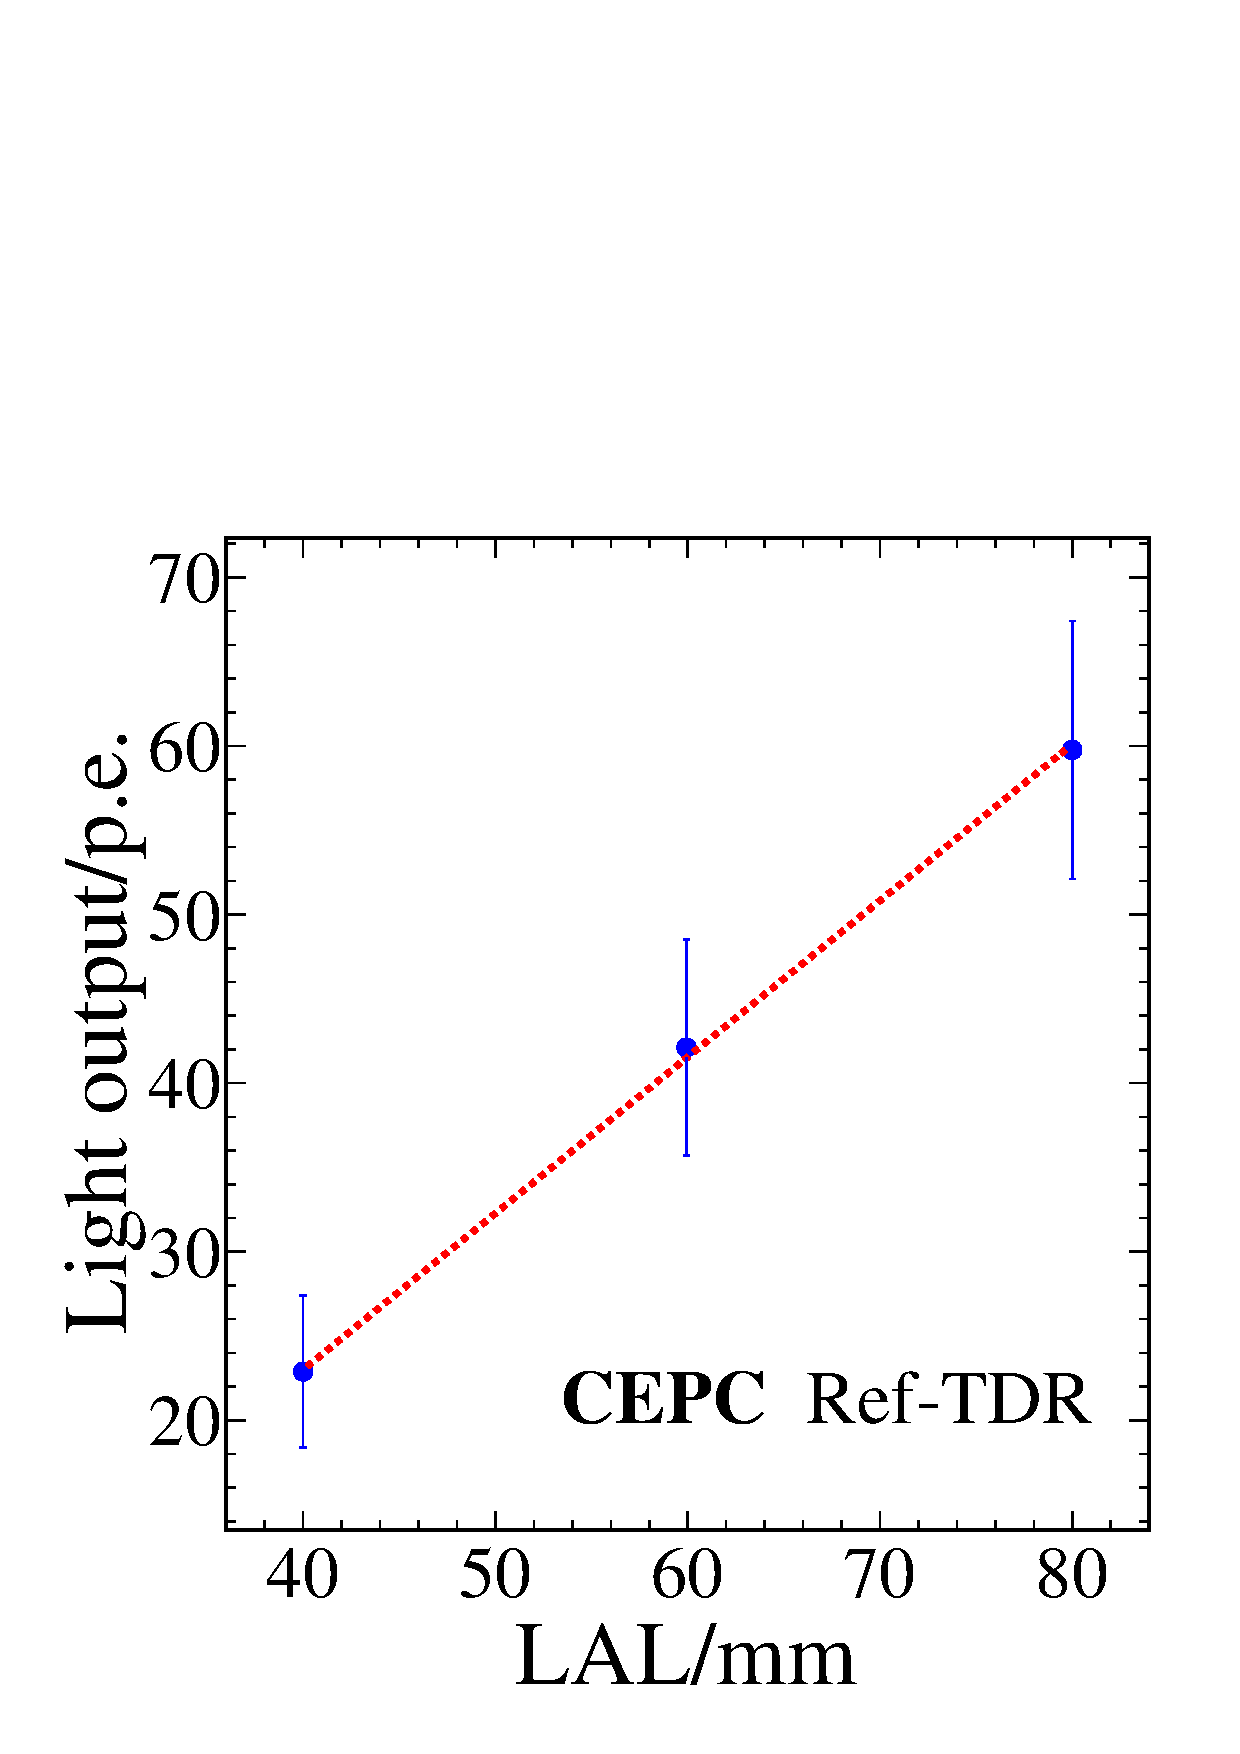
\includegraphics[width=\linewidth]{attenuation_fit.pdf}
  \caption{}
\end{subfigure}
\caption{(a)~Simulated light-output distribution of a GS cell with
\SI{60}{mm} attenuation length ($42.05\pm0.01$~\peMIP).
(b)~Fitted light-output MPV versus attenuation length (40, 60, and
\SI{80}{mm}).}
\label{fig:SiPM_MIPmap}
\end{figure}

Validation studies (Figure~\ref{fig:SiPM_SimValid}) reveal simulated
fast and slow scintillation-time components of \SI{96}{ns} and
\SI{1445}{ns}, somewhat longer than the measured reference values
(\SI{60}{ns} and \SI{500}{ns}; Table~\ref{tab:GS1}), indicating that
Geant4 fine-tuning with experimental GFO data is still required.
The simulated deposited-energy distribution for \SI{5}{GeV} muons yields
an MPV of approximately \SI{7.3}{MeV} per MIP, in good agreement with
expectation.

\begin{figure}[htbp]
\centering
\begin{subfigure}{0.43\textwidth}
  \centering
  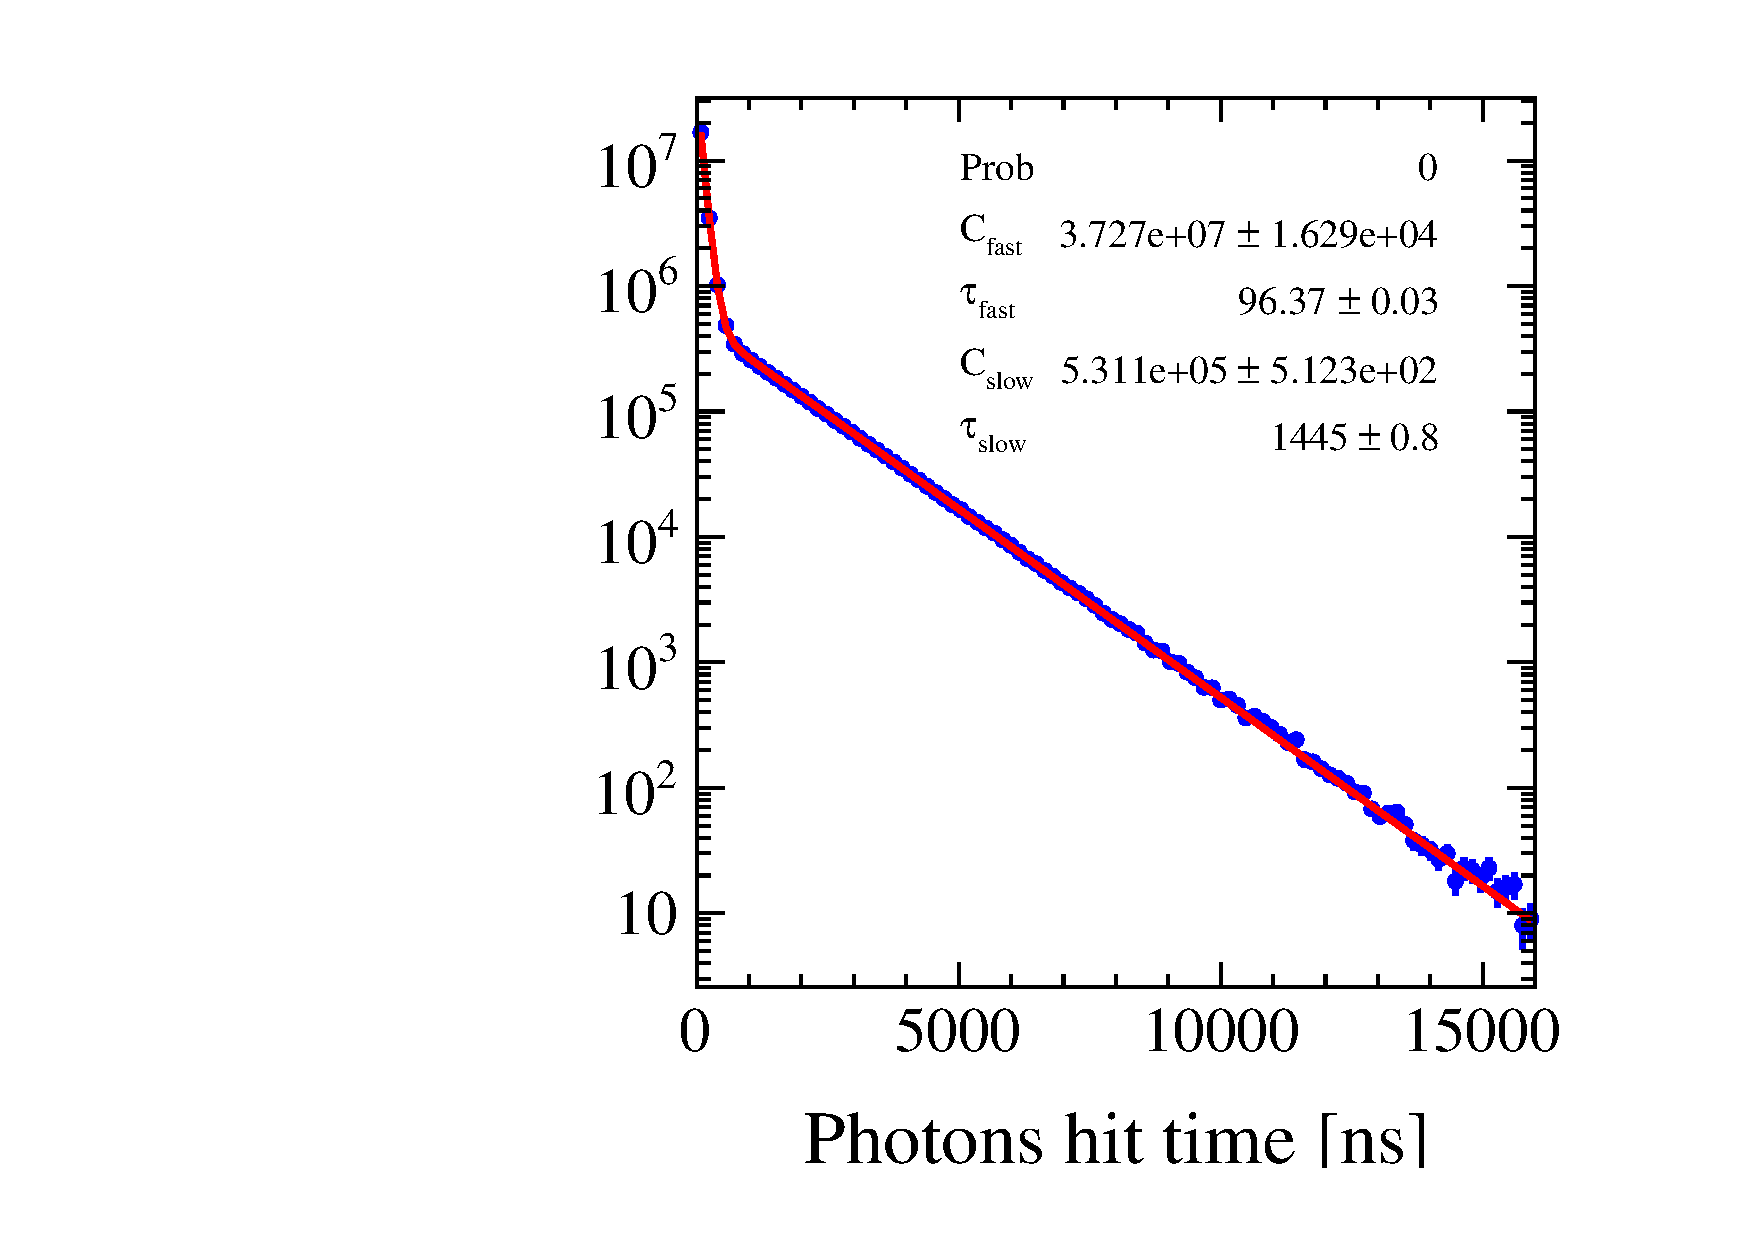
\includegraphics[width=\linewidth]{timeSpe.pdf}
  \caption{}
\end{subfigure}\hfill
\begin{subfigure}{0.38\textwidth}
  \centering
  \includegraphics[width=\linewidth]{Edp.pdf}
  \caption{}
\end{subfigure}
\caption{Simulation validation: (a)~scintillation-time distribution
(fast and slow components); (b)~muon deposited energy in a
\SI{10}{mm}-thick GS cell.}
\label{fig:SiPM_SimValid}
\end{figure}

%% ====================================================================
\section{Measurements and calibration}
\label{sec:measurements}
%% ====================================================================

%% --------------------------------------------------------------------
\subsection{Single-cell measurements}
\label{subsec:cellmeas}
%% --------------------------------------------------------------------

The effective light output of \cellsize GS cells was evaluated in three
independent measurement campaigns:
\begin{enumerate}
\item \SI{662}{keV} $\gamma$-rays from a $^{137}$Cs radioactive source;
\item cosmic-ray muons (expected energy deposition
  \SI{7.7}{MeV}/MIP);
\item \SI{5}{GeV} electron beams at KEK\@.
\end{enumerate}
In each case the SiPM sensor was mounted at the cell centre on a
readout board with a pre-amplifier.
Comparative tests of enhanced-specular-reflector (ESR) and Teflon
reflective films showed that Teflon provides approximately 20\% higher
effective reflectivity~\cite{Janecek:2012qit}, attributed to its
diffuse reflectivity and superior optical contact with the glass
surface; all measurements therefore employ Teflon wrapping.

\paragraph{$^{137}$Cs measurement.}
Using the HPK~S14160-3050HS SiPM (spectrum-weighted PDE~44.5\%), the
MPV for \SI{662}{keV} $\gamma$-rays is 12.9~p.e.
Scaling to the expected \SI{7.7}{MeV} MIP energy deposition yields an
equivalent light output of approximately $150$~\peMIP.

\paragraph{Cosmic-ray measurement.}
A trigger formed by two plastic-scintillator panels selects
through-going muons.
With the HPK~S13360-3050PE SiPM (spectrum-weighted PDE~32.5\%) the
measured light output is $63.6\pm0.5$~\peMIP
(Figure~\ref{fig:SiPM_Celltest}b).

\paragraph{Electron beam test at KEK.}
A Landau fit to the \SI{5}{GeV} electron spectrum measured with the
NDL~EQR20-11-3030 SiPM (spectrum-weighted PDE~42.5\%) yields an MPV of
$157.6\pm2.9$~\peMIP (Figure~\ref{fig:SiPM_Celltest}c).

\begin{figure}[htbp]
\centering
\begin{subfigure}{0.49\textwidth}
  \centering
  \includegraphics[width=\linewidth]{GS-SiPM-Cs137-Teflon.pdf}
  \caption{}
\end{subfigure}\hfill
\begin{subfigure}{0.49\textwidth}
  \centering
  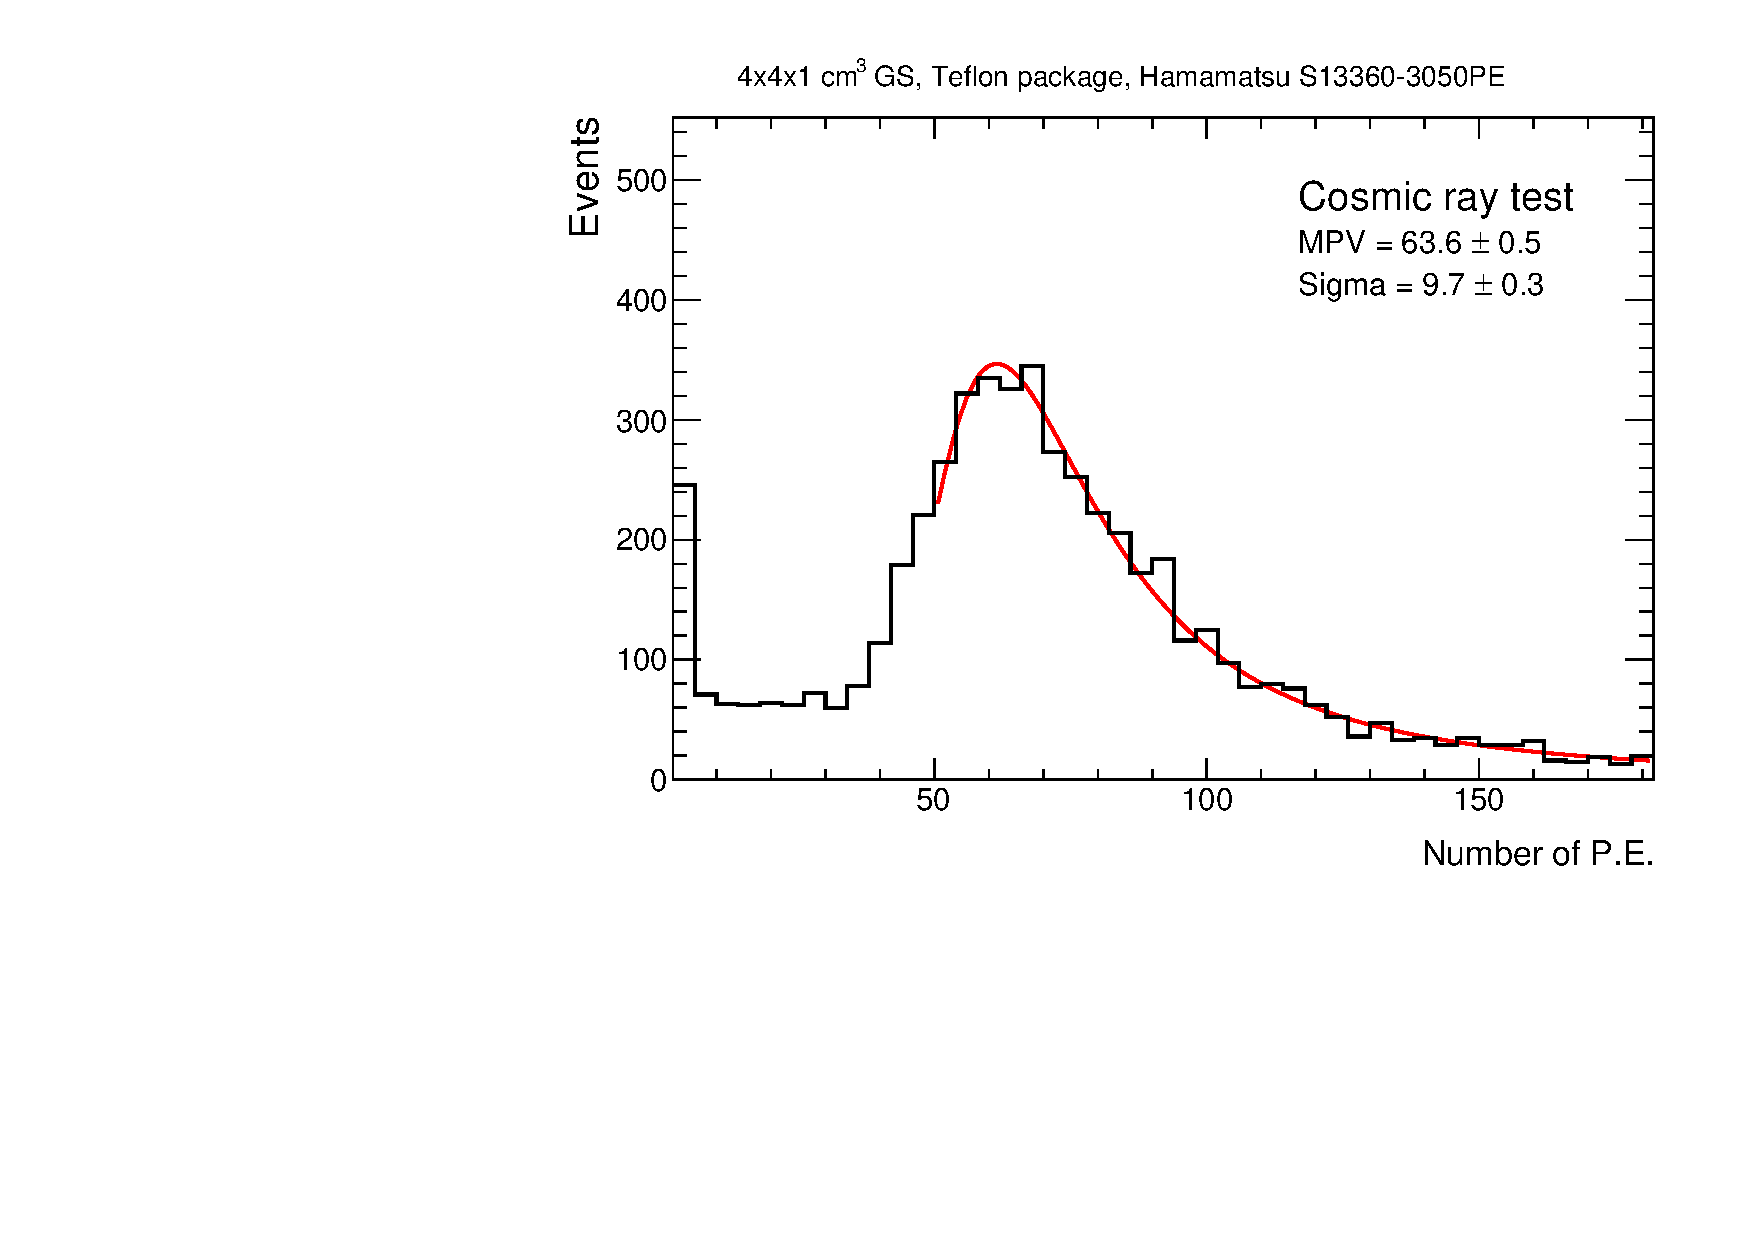
\includegraphics[width=\linewidth]{Cosmic_GSSiPM_SJTU_Teflon.pdf}
  \caption{}
\end{subfigure}

\vspace{0.3cm}

\begin{subfigure}{0.49\textwidth}
  \centering
  \includegraphics[width=\linewidth]{KEK_BeamTest_Electron.png}
  \caption{}
\end{subfigure}
\caption{Single-cell measurement results (\cellsize GS with SiPM
readout).
(a)~ADC spectrum with $^{137}$Cs source (HPK~S14160-3050HS).
(b)~Cosmic-ray test (HPK~S13360-3050PE): $63.6\pm0.5$~\peMIP.
(c)~Response to \SI{5}{GeV} electrons at KEK (NDL~EQR20-11-3030):
Landau-fit MPV $157.6\pm2.9$~\peMIP.}
\label{fig:SiPM_Celltest}
\end{figure}

The factor-of-three increase in light output for \SI{5}{GeV} electrons
relative to cosmic muons arises from the fundamentally different energy
deposition mechanisms.
A cosmic muon deposits energy primarily through ionisation
(${\sim}\SI{7.7}{MeV\per MIP}$), whereas a \SI{5}{GeV} electron
(well above the critical energy $E_{c}\sim\SI{10}{MeV}$ for GS)
predominantly loses energy via bremsstrahlung, initiating an
electromagnetic shower whose localised energy density greatly exceeds
that of a minimum-ionising track.

The measured cosmic-ray light output of 64~\peMIP exceeds the simulated
value of 42~\peMIP (Section~\ref{subsec:optsim}).
This discrepancy likely originates from uncalibrated Geant4 optical
parameters for the newly developed GFO material.
Improving the simulation accuracy remains a high priority.

%% --------------------------------------------------------------------
\subsection{Calibration strategy}
\label{subsec:calibration}
%% --------------------------------------------------------------------

\subsubsection{Physics-process calibration}
\label{sssec:physcalib}

The global calibration of the GS-HCAL exploits MIP signals from prompt
muons in $e^{+}e^{-}\to Z\to\mu^{+}\mu^{-}$ events.
Figure~\ref{fig:kinematic_mumu} shows the kinematic distributions at
$\sqrt{s}=\SI{91.2}{GeV}$.
At design luminosity this process occurs at a rate of \SI{584}{Hz}.
A conservative estimate yields 47~events per hour within a
$\Delta\phi\times\Delta\!\cos\theta=0.018\times0.018$ acceptance window
corresponding to one GS cell at the central-barrel HCAL surface.
Assuming bi-weekly $Z$-mode calibration runs (\SI{16}{h/day}),
$4.71\times10^{8}$ di-muon events can be collected, achieving
approximately 1\% statistical precision.

\begin{figure}[htbp]
\centering
\begin{subfigure}{0.32\textwidth}
  \centering
  \includegraphics[width=\linewidth]{Fig8_mumu_cosTheta.pdf}
  \caption{}
\end{subfigure}\hfill
\begin{subfigure}{0.32\textwidth}
  \centering
  \includegraphics[width=\linewidth]{Fig8_mumu_phi.pdf}
  \caption{}
\end{subfigure}\hfill
\begin{subfigure}{0.32\textwidth}
  \centering
  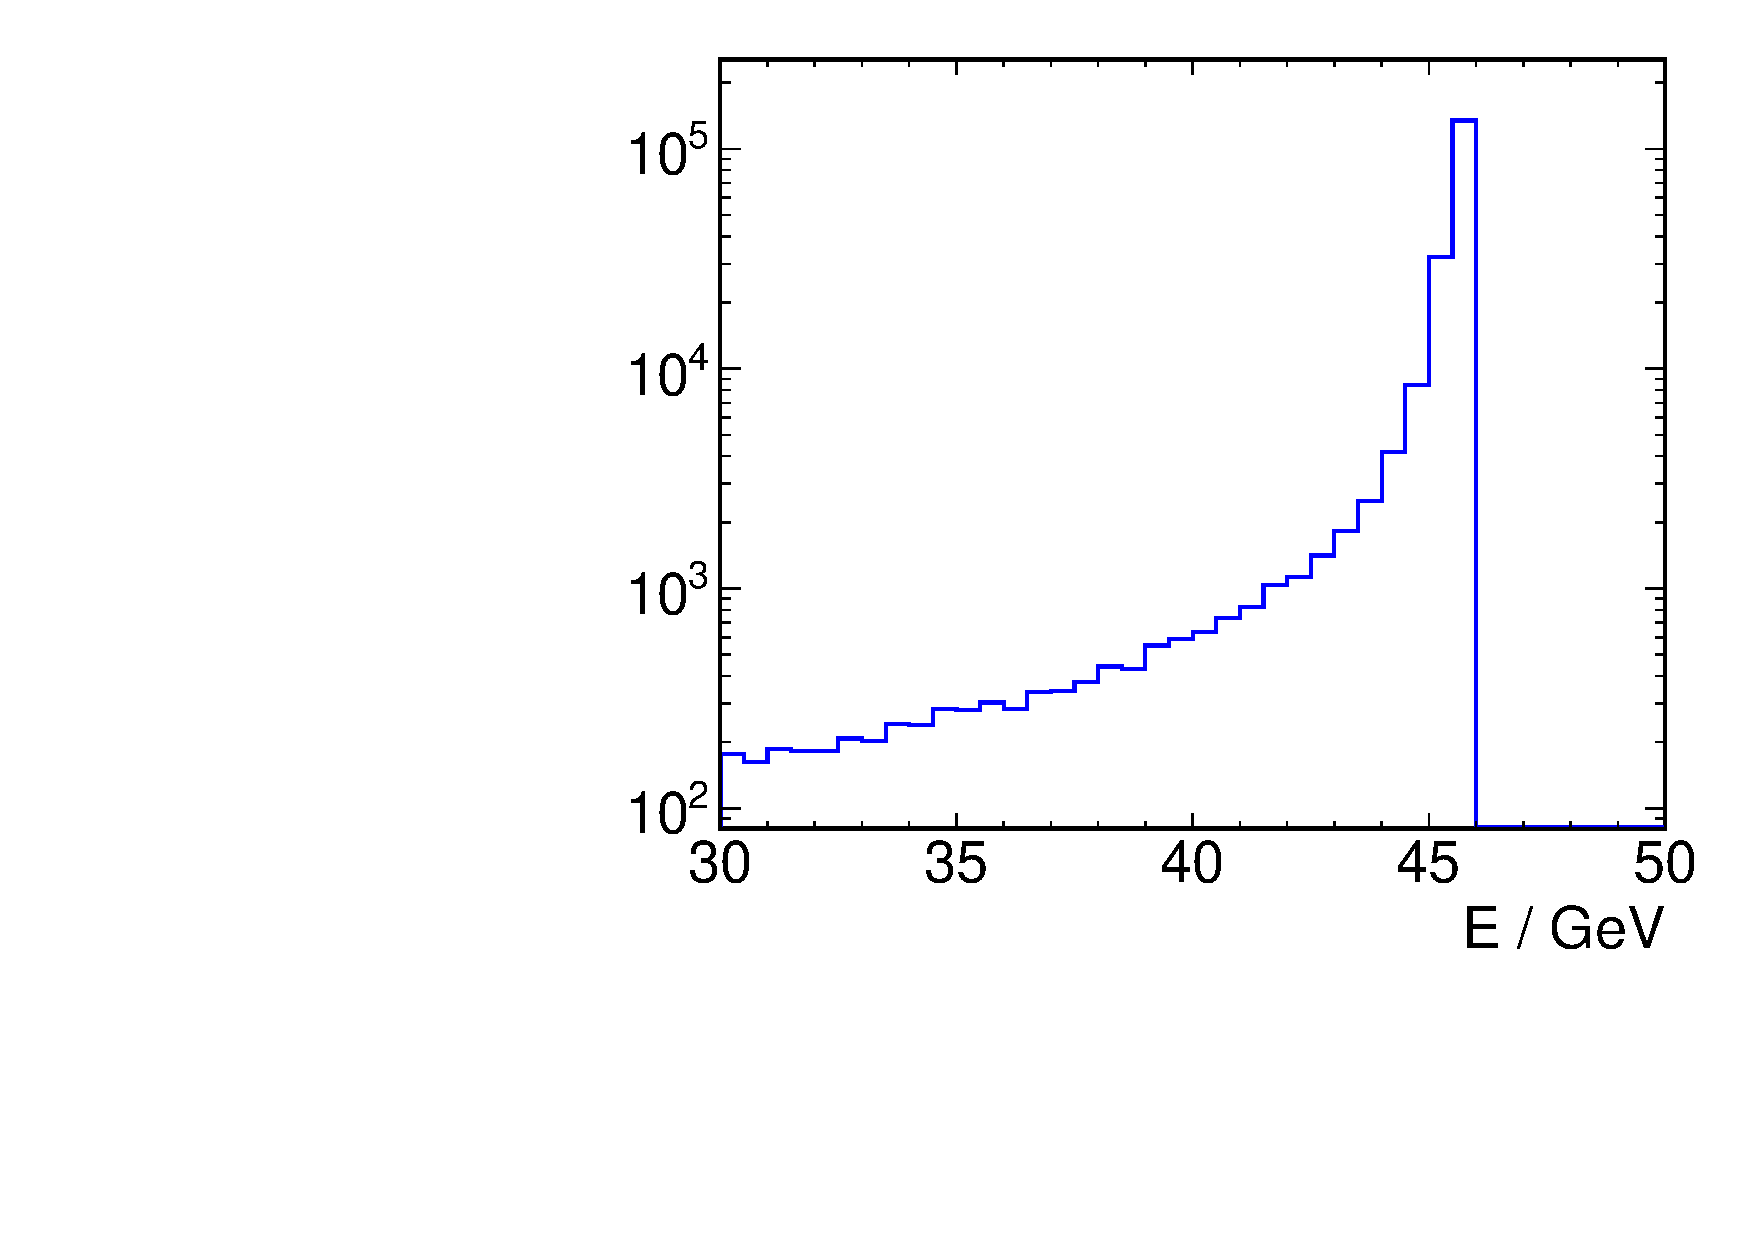
\includegraphics[width=\linewidth]{Fig8_mumu_E.pdf}
  \caption{}
\end{subfigure}
\caption{Generator-level distributions of (a)~$\cos\theta$, (b)~$\phi$,
and (c)~energy of muons in $e^{+}e^{-}\to\mu^{+}\mu^{-}$ at
$\sqrt{s}=\SI{91.2}{GeV}$.}
\label{fig:kinematic_mumu}
\end{figure}

The dominant $Z$-pole process $e^{+}e^{-}\to Z\to q\bar{q}$ provides
resonant dijets for combined ECAL and HCAL calibration via the
reconstructed invariant mass $m_{jj}$ (Figure~\ref{fig:kinematic_zjj}).

\begin{figure}[htbp]
\centering
\includegraphics[width=0.50\textwidth]{Mjj_eeuu_91.pdf}
\caption{Distribution of dijet invariant mass from $Z\to q\bar{q}$ at
$\sqrt{s}=\SI{91.2}{GeV}$.}
\label{fig:kinematic_zjj}
\end{figure}

Additional calibration using hadronic $\tau$ decays in
$Z\to\tau^{+}\tau^{-}$ and isolated hadrons within jets provides
complementary $E/p$ monitoring of the HCAL response over time.

\subsubsection{Hardware calibration}
\label{sssec:hwcalib}

The hardware calibration system comprises two complementary approaches:
(i)~MIP inter-calibration using cosmic rays or muon beams, and (ii)~an
online LED-based monitoring system.
The LED system (Figure~\ref{fig:Calibration-2n}) employs a centrally
located LED with optical-fibre distribution to multiple cells, enabling
continuous tracking of pedestal levels, gain characteristics, and
response linearity.

\begin{figure}[htbp]
\centering
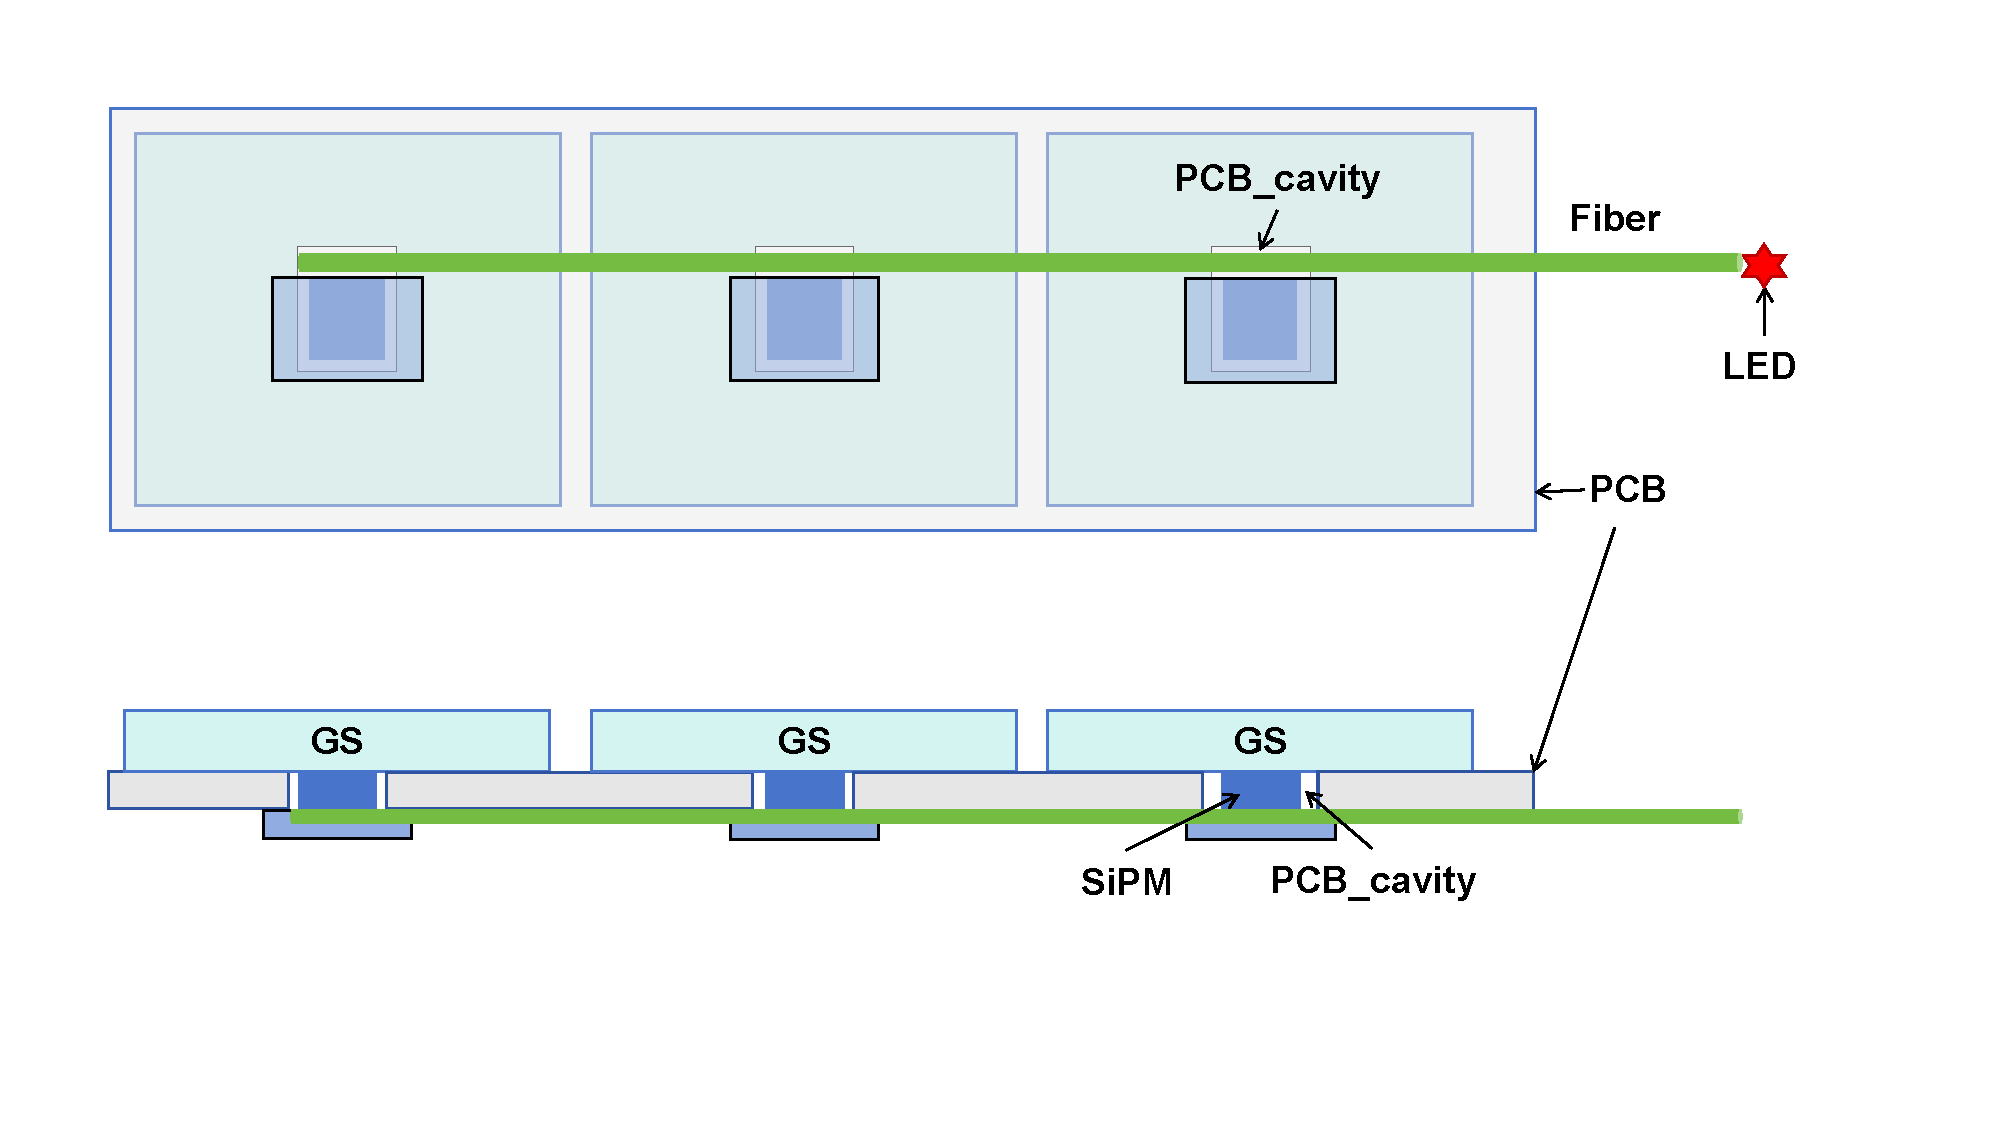
\includegraphics[width=0.68\textwidth]{Calibration-2n.pdf}
\caption{Schematic of the GS-HCAL LED calibration system showing
optical-fibre connections between adjacent cells: top~view~(a) and
side~view~(b).}
\label{fig:Calibration-2n}
\end{figure}

%% ====================================================================
\section{Readout electronics and prototype}
\label{sec:electronics}
%% ====================================================================

%% --------------------------------------------------------------------
\subsection{Readout electronics}
\label{subsec:roe}
%% --------------------------------------------------------------------

The GS-HCAL requires front-end electronics (FEE) for more than five
million SiPM channels.
The readout chain comprises a stable, low-noise bias-voltage supply;
a charge-sensitive pre-amplifier; a shaping stage optimised for
signal-to-noise ratio; discriminators for photon counting; and
analogue-to-digital converters (ADCs).
Table~\ref{tab:SiPM-tab3} lists the key specifications.

\begin{table}[htbp]
\centering
\caption{SiPM-driven requirements for the readout electronics.}
\label{tab:SiPM-tab3}
\begin{tabular}{ll}
\toprule
\textbf{Parameter} & \textbf{Requirement} \\
\midrule
Charge dynamic range       & \SI{0.8}{pC}--\SI{800}{pC} (0.1--100~MIP) \\
Charge resolution          & 10\% of 1.0~MIP \\
SiPM capacitance           & $\leq\SI{100}{pF}$ \\
SiPM gain                  & $\geq5\times10^{5}$ \\
Average event rate/channel & \SI{2}{kHz} \\
Maximum event rate/channel & \SI{50}{kHz} \\
Typical signal amplitude   & 2--3~mV/p.e. \\
\bottomrule
\end{tabular}
\end{table}

An interim FEE solution~\cite{Wang:2023ffl} was developed for SiPM
characterisation and prototype testing, as no commercial option met the
requirements.
The pre-amplifier (Figure~\ref{fig:SiPM_FEE}) achieves a gain of
$\pm\SI{20}{V/V}$, bandwidth of \SI{400}{MHz}, and baseline noise of
$300\,\mu\mathrm{V}_\mathrm{RMS}$ with \SI{50}{\ohm} input impedance.
Figure~\ref{fig:SiPM_FEE}(e) shows a typical SiPM waveform, and
Figure~\ref{fig:SiPM_FEE}(f) the ADC spectrum of dark noise with
well-separated photoelectron peaks.

\begin{figure}[htbp]
\centering
\includegraphics[width=0.95\textwidth]{SiPM_FEE.pdf}
\caption{Pre-amplifier for the GS-HCAL SiPM readout.
(a)~Single-channel PCB coupled to a GS cell.
(b)~Schematic diagram.
(c,\,d)~Performance characteristics.
(e)~Waveform of a \sipmsize NDL SiPM (EQR20-11-3030D-S).
(f)~ADC spectrum of SiPM dark noise.}
\label{fig:SiPM_FEE}
\end{figure}

%% --------------------------------------------------------------------
\subsection{Prototype design and beam-test programme}
\label{subsec:prototype}
%% --------------------------------------------------------------------

A GS-HCAL prototype is under construction following the single-layer
design of Section~\ref{subsec:onelayer}.
The prototype is a steel-scintillator sandwich of
$52.0\times52.0\times130.6$~cm$^{3}$ (${\approx}\SI{0.6}{m^{3}}$),
containing 8112~GS cells in 48~layers (${\approx}6\,\lambdaI$).
Each layer has a $13\times13$ array of \cellsize cells, each coupled to
a \sipmsize SiPM\@.  The steel absorber plates are S304 stainless steel
(\SI{9.8}{mm} thick).

Geant4 simulations with \SI{80}{GeV} $\pi^{-}$ beams
(Figure~\ref{fig:prototype-sim-energy}) show that the
$13\times13\times48$ configuration achieves 95\% energy containment.
Figure~\ref{fig:prototype-sim-resolution} presents the projected
energy resolution and linearity.
The prototype is expected to achieve a single-hadron energy resolution
of approximately $45\%/\sqrt{E}\oplus8\%$, degraded relative to the
full detector owing to the limited lateral size; this performance is
nonetheless sufficient to validate the key GS technology and
reconstruction algorithms.

\begin{figure}[htbp]
\centering
\includegraphics[width=0.50\linewidth]{Edep_module_80GeV.pdf}
\caption{Simulated deposited energy in prototypes of different lateral
sizes for \SI{80}{GeV} $\pi^{-}$; the $13\times13\times48$
configuration achieves ${\approx}95\%$ containment.}
\label{fig:prototype-sim-energy}
\end{figure}

\begin{figure}[htbp]
\centering
\begin{subfigure}{0.40\textwidth}
  \centering
  \includegraphics[width=\linewidth]{prototype_simulation-13}
  \caption{}
\end{subfigure}\hfill
\begin{subfigure}{0.40\textwidth}
  \centering
  \includegraphics[width=\linewidth]{prototype_simulation-linear.jpg}
  \caption{}
\end{subfigure}
\caption{Simulated (a)~energy resolution and (b)~energy linearity of
the GS-HCAL prototype.}
\label{fig:prototype-sim-resolution}
\end{figure}

The construction and testing programme proceeds in phases:
\begin{itemize}
\item A $3\times3\times7$ mini-prototype is under construction for
  initial beam tests at CERN in October~2025.
\item The full 8112-channel prototype is scheduled for completion by
  end-2026, with cosmic-ray tests at IHEP and beam tests preferably
  in~2027.
\item The beam-test platform provides $\pm\SI{25}{cm}$ positioning
  accuracy ($<\SI{1}{mm}$ precision), $\pm30^{\circ}$ rotation, and
  \SI{5}{t} capacity.
\item Alternative test sites include the China Spallation Neutron
  Source (CSNS, \SI{1.6}{GeV} proton beam) and the facility at the
  University of Tokyo.
\end{itemize}

Key subsystems include: blue-LED calibration for SiPM-gain monitoring;
a new ASIC with \SI{15}{mW/channel} power consumption; TiO$_{2}$ and
Teflon reflective coating; and a water-based cooling system with
precisely regulated flow rate and temperature.

%% ====================================================================
\section{Simulation and performance}
\label{sec:simperf}
%% ====================================================================

%% --------------------------------------------------------------------
\subsection{Simulation setup}
\label{subsec:simsetup}
%% --------------------------------------------------------------------

The intrinsic energy linearity and resolution of the GS-HCAL are
evaluated using Geant4 simulation within the CEPCSW
framework~\cite{CEPCStudyGroup:2018ghi}, with all inner sub-detectors
removed.
A digitisation model incorporates the following effects:
\begin{itemize}
\item \textbf{Birks' constant:} a preliminary value
  $k_{B}=\SI{0.01}{cm/MeV}$ is used; a dedicated measurement with
  heavy-ion beams is being planned.
\item \textbf{Light yield:} based on GS measurements the intrinsic MIP
  light yield is \SI{1500}{\phMeV}, giving a detected effective light
  output of $\geq60$~\peMIP.
\item \textbf{Attenuation length:} \SI{6}{cm} (current measured value).
\item \textbf{Readout threshold:} 0.1~MIP, determined by scanning its
  impact on the energy resolution.
\item \textbf{SiPM response} and electronic-system characteristics.
\end{itemize}

%% --------------------------------------------------------------------
\subsection{Single-hadron energy resolution}
\label{subsec:hadronres}
%% --------------------------------------------------------------------

The energy resolution for single hadrons is parametrised as
\begin{equation}
\label{eq:eres}
\frac{\sigma_{E}}{E} = \frac{a}{\sqrt{E}} \oplus b,
\end{equation}
where $a$ denotes the stochastic term and $b$ the constant term.
With the full digitisation model the GS-HCAL yields
\begin{equation}
\frac{\sigma_{E}}{E} = \frac{29.8\%}{\sqrt{E\,[\text{GeV}]}}
\oplus 6.5\%,
\end{equation}
with energy non-linearity within 2\% (Figure~\ref{fig:Eres_HCAL_final}).
The default hadronic-physics list is \texttt{QGSP\_BERT}.
The stochastic term substantially outperforms conventional HCALs, which
typically achieve ${\sim}60\%/\sqrt{E}\oplus3\%$.
The comparatively large constant term is attributed to longitudinal
leakage in the $6\,\lambdaI$ design and is expected to be further
reduced by software compensation and PFA
techniques~\cite{Simon:2009bt,Rolph:2022eba,CALICE:2024imr,Liu:2025hgf}.

\begin{figure}[htbp]
\centering
\begin{subfigure}{0.45\linewidth}
  \centering
  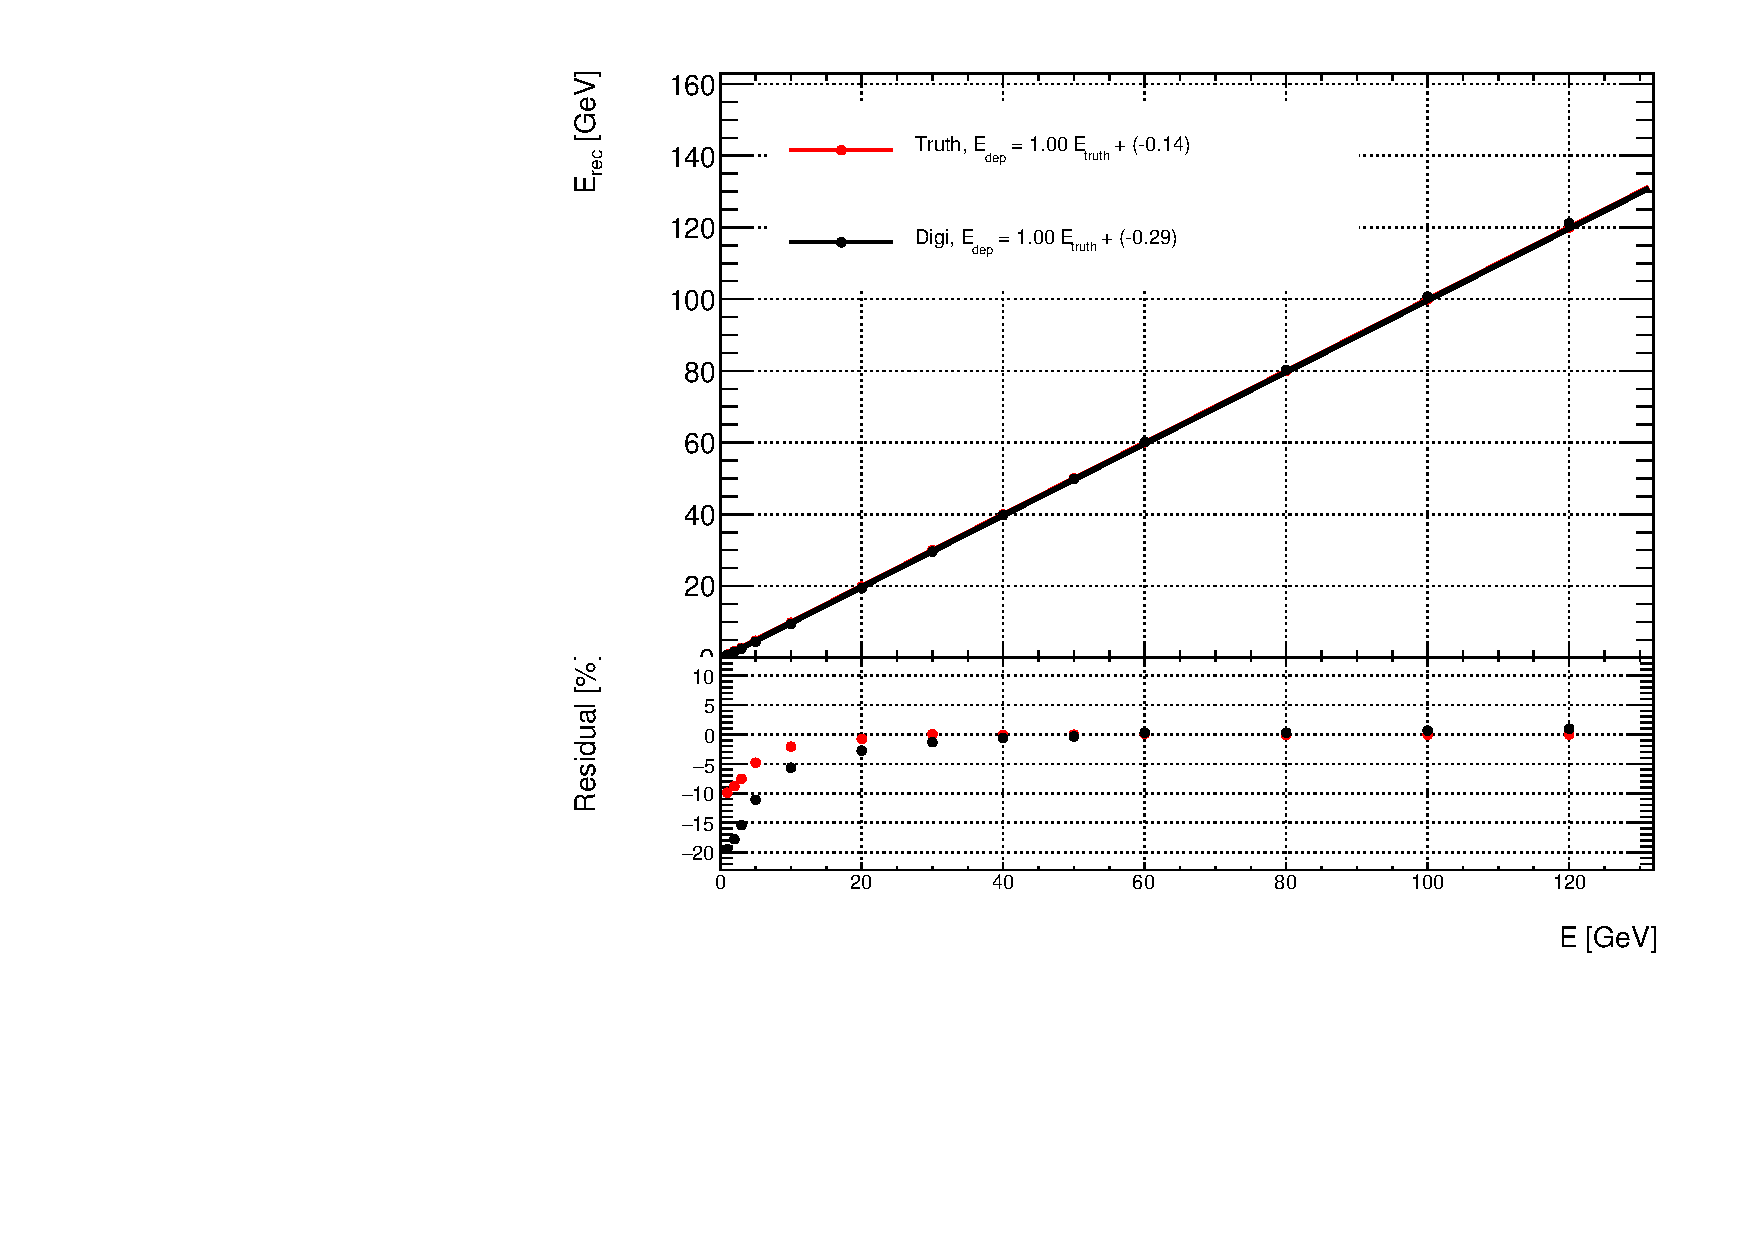
\includegraphics[width=\linewidth]{Elin_digi.pdf}
  \caption{}
\end{subfigure}\hfill
\begin{subfigure}{0.45\linewidth}
  \centering
  \includegraphics[width=\linewidth]{Eres_digi.pdf}
  \caption{}
\end{subfigure}
\caption{(a)~Energy linearity and (b)~energy resolution of the GS-HCAL
from the full digitisation model.}
\label{fig:Eres_HCAL_final}
\end{figure}

In the CEPC collision environment (Figure~\ref{fig:Ehad_CEPC}), more
than 98\% of hadronic final-state objects have energies below
\SI{60}{GeV}, a regime in which the GS-HCAL achieves optimal resolution.

\begin{figure}[htbp]
\centering
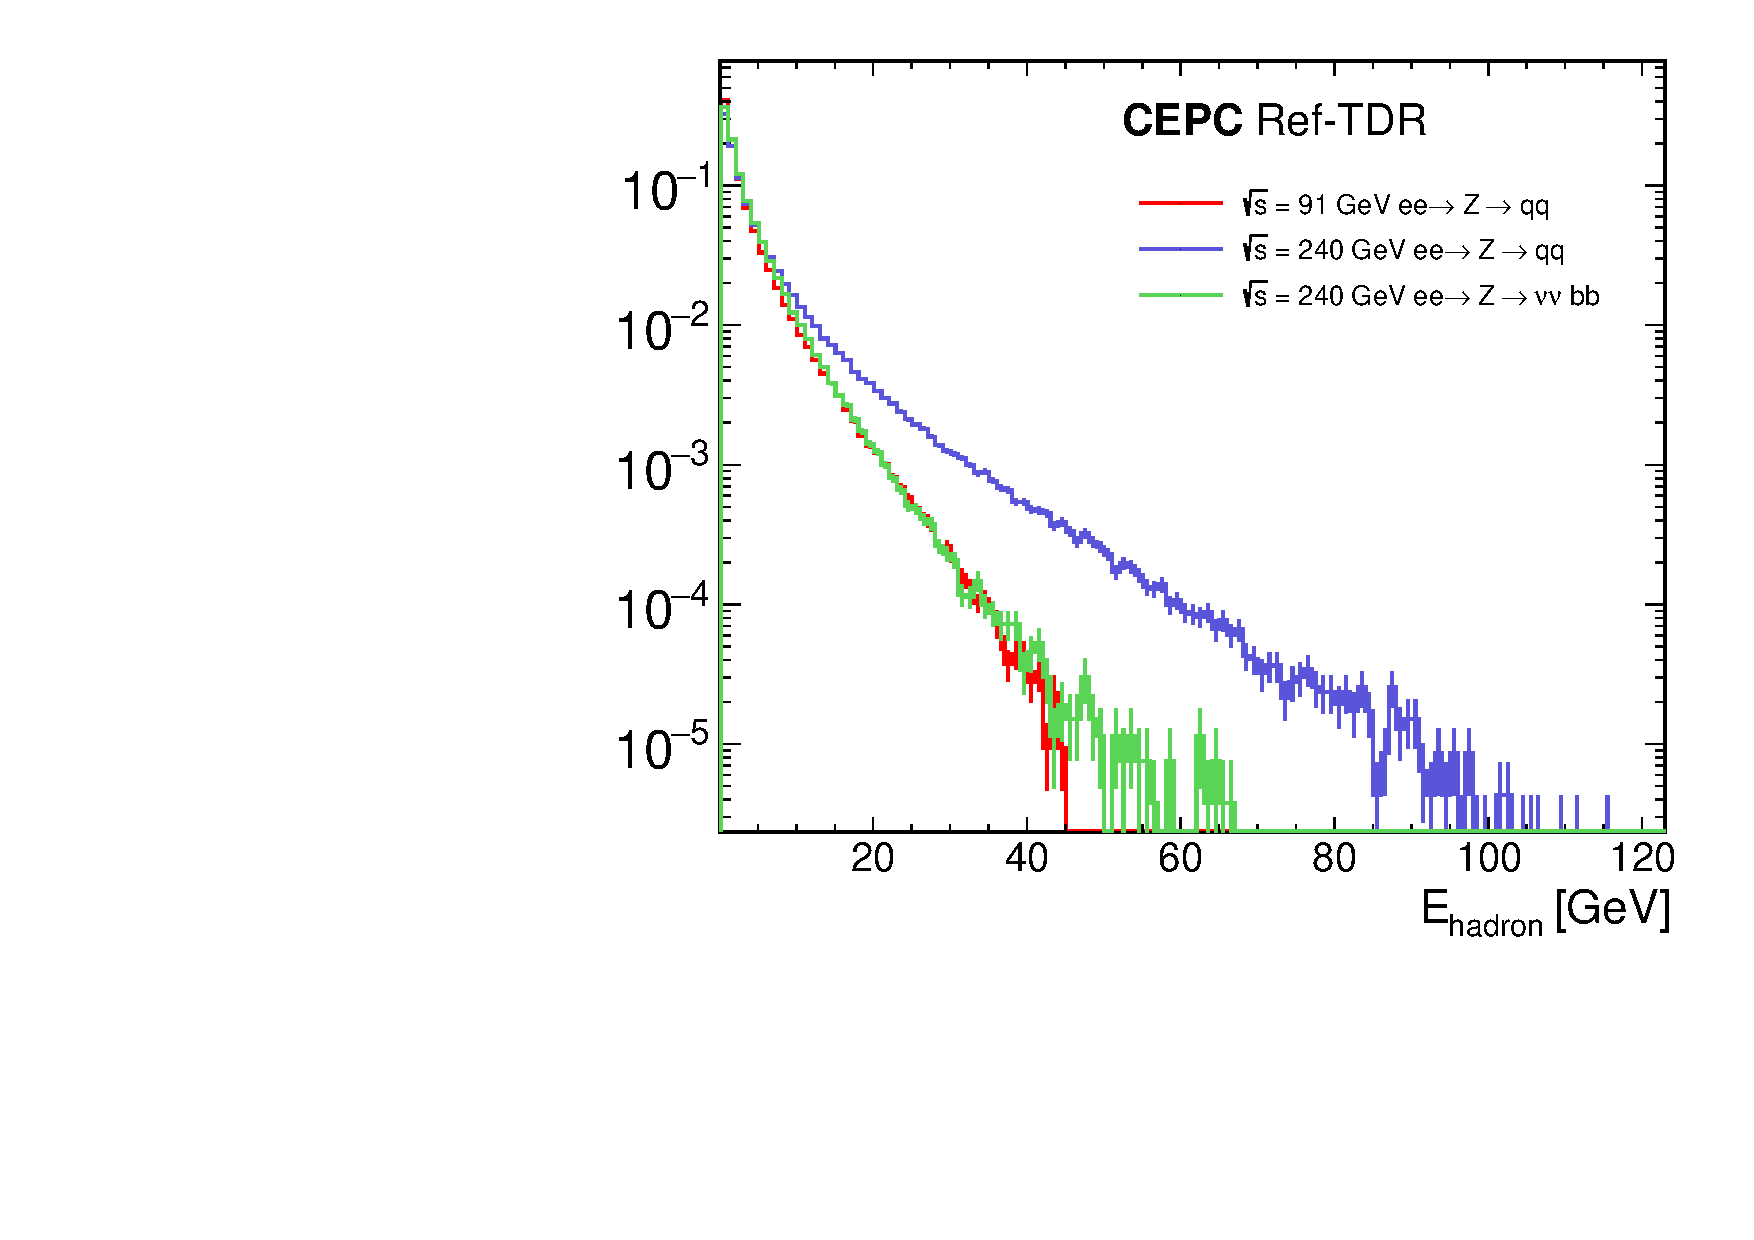
\includegraphics[width=0.50\linewidth]{Ehadrons.pdf}
\caption{Energy distribution of hadronic objects in the most energetic
CEPC $e^{+}e^{-}$ processes.}
\label{fig:Ehad_CEPC}
\end{figure}

A systematic parameter scan (Figure~\ref{fig:Eres_vs_parameters})
quantifies the sensitivity of the energy resolution to
(a)~light output and threshold, (b)~GS attenuation length, and
(c)~Birks' constant, confirming that these parameters are most
influential in the low-energy regime.

\begin{figure}[htbp]
\centering
\begin{subfigure}{0.48\linewidth}
  \centering
  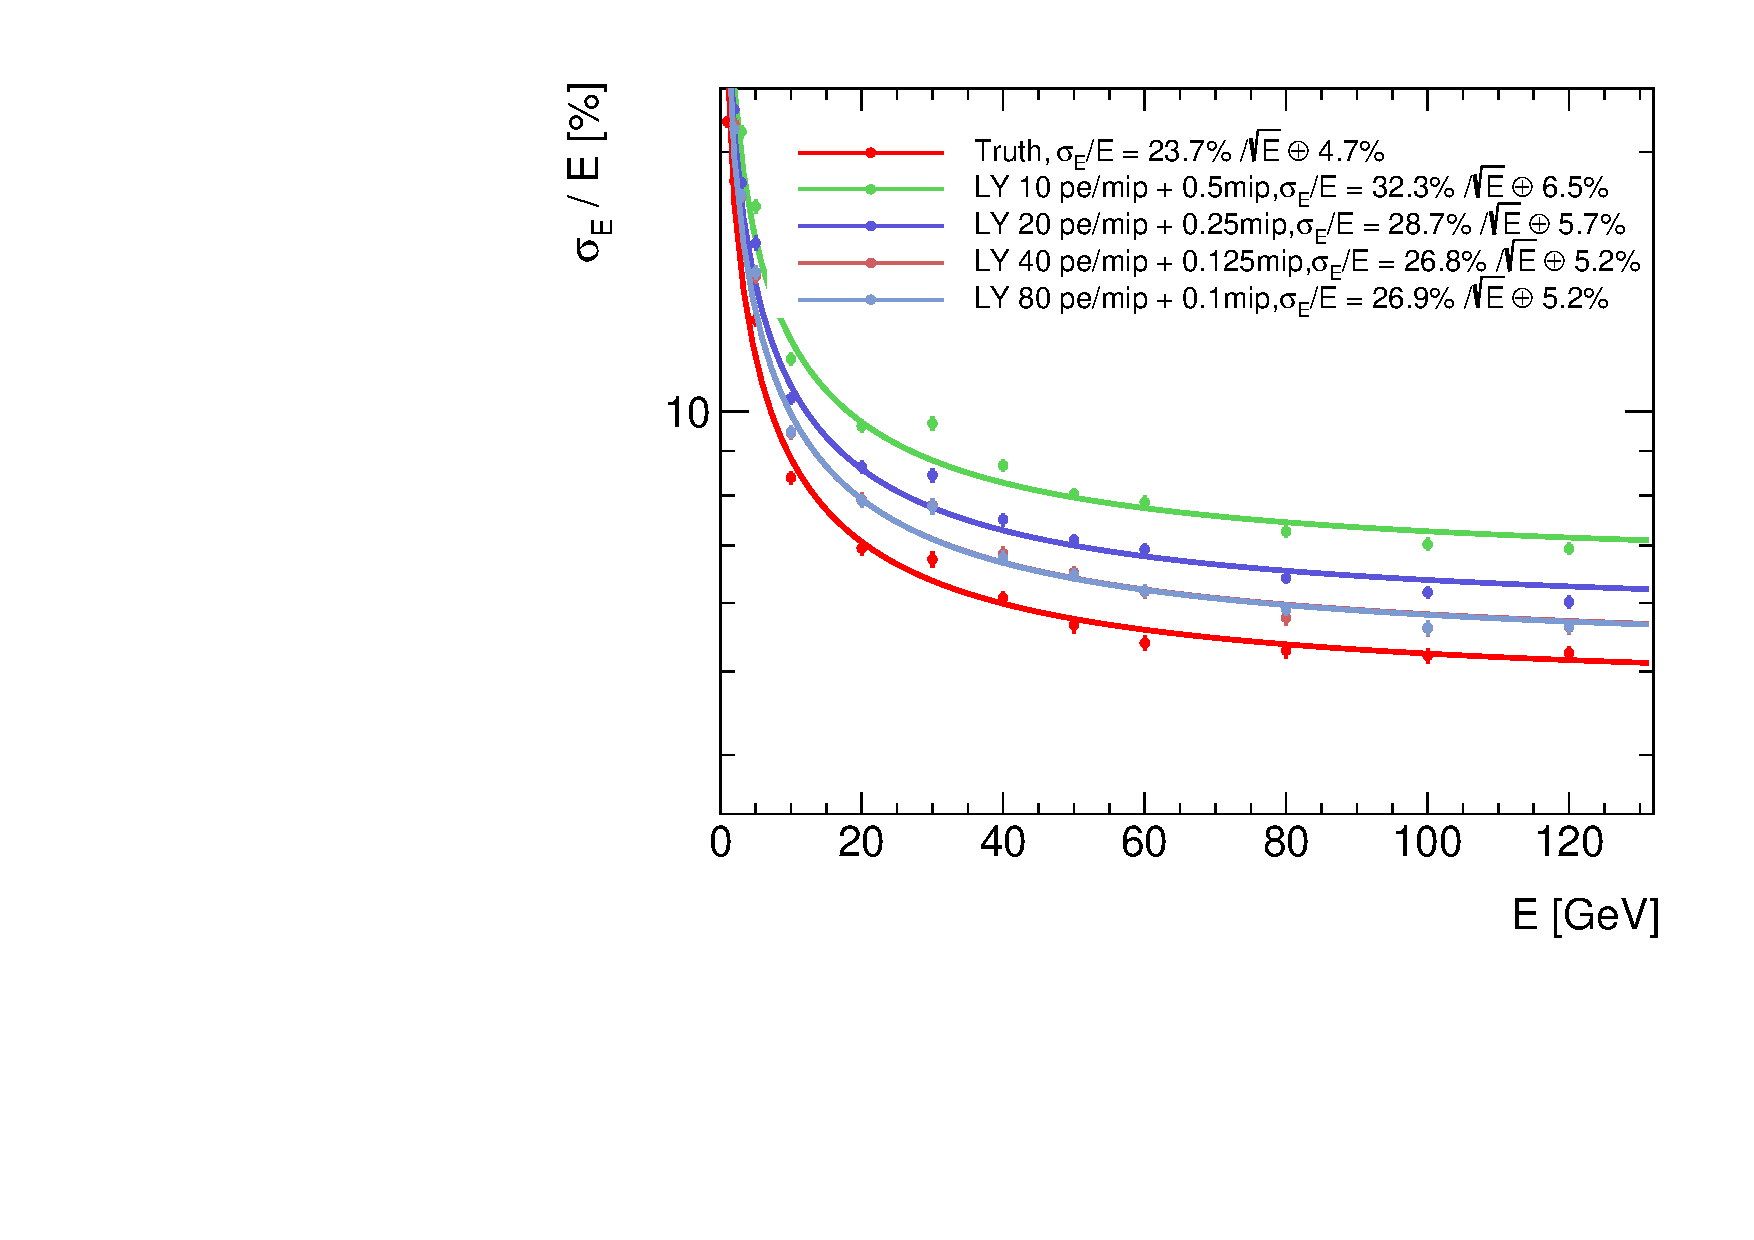
\includegraphics[width=\linewidth]{Eres_LYTh_Log.pdf}
  \caption{}
\end{subfigure}\hfill
\begin{subfigure}{0.48\linewidth}
  \centering
  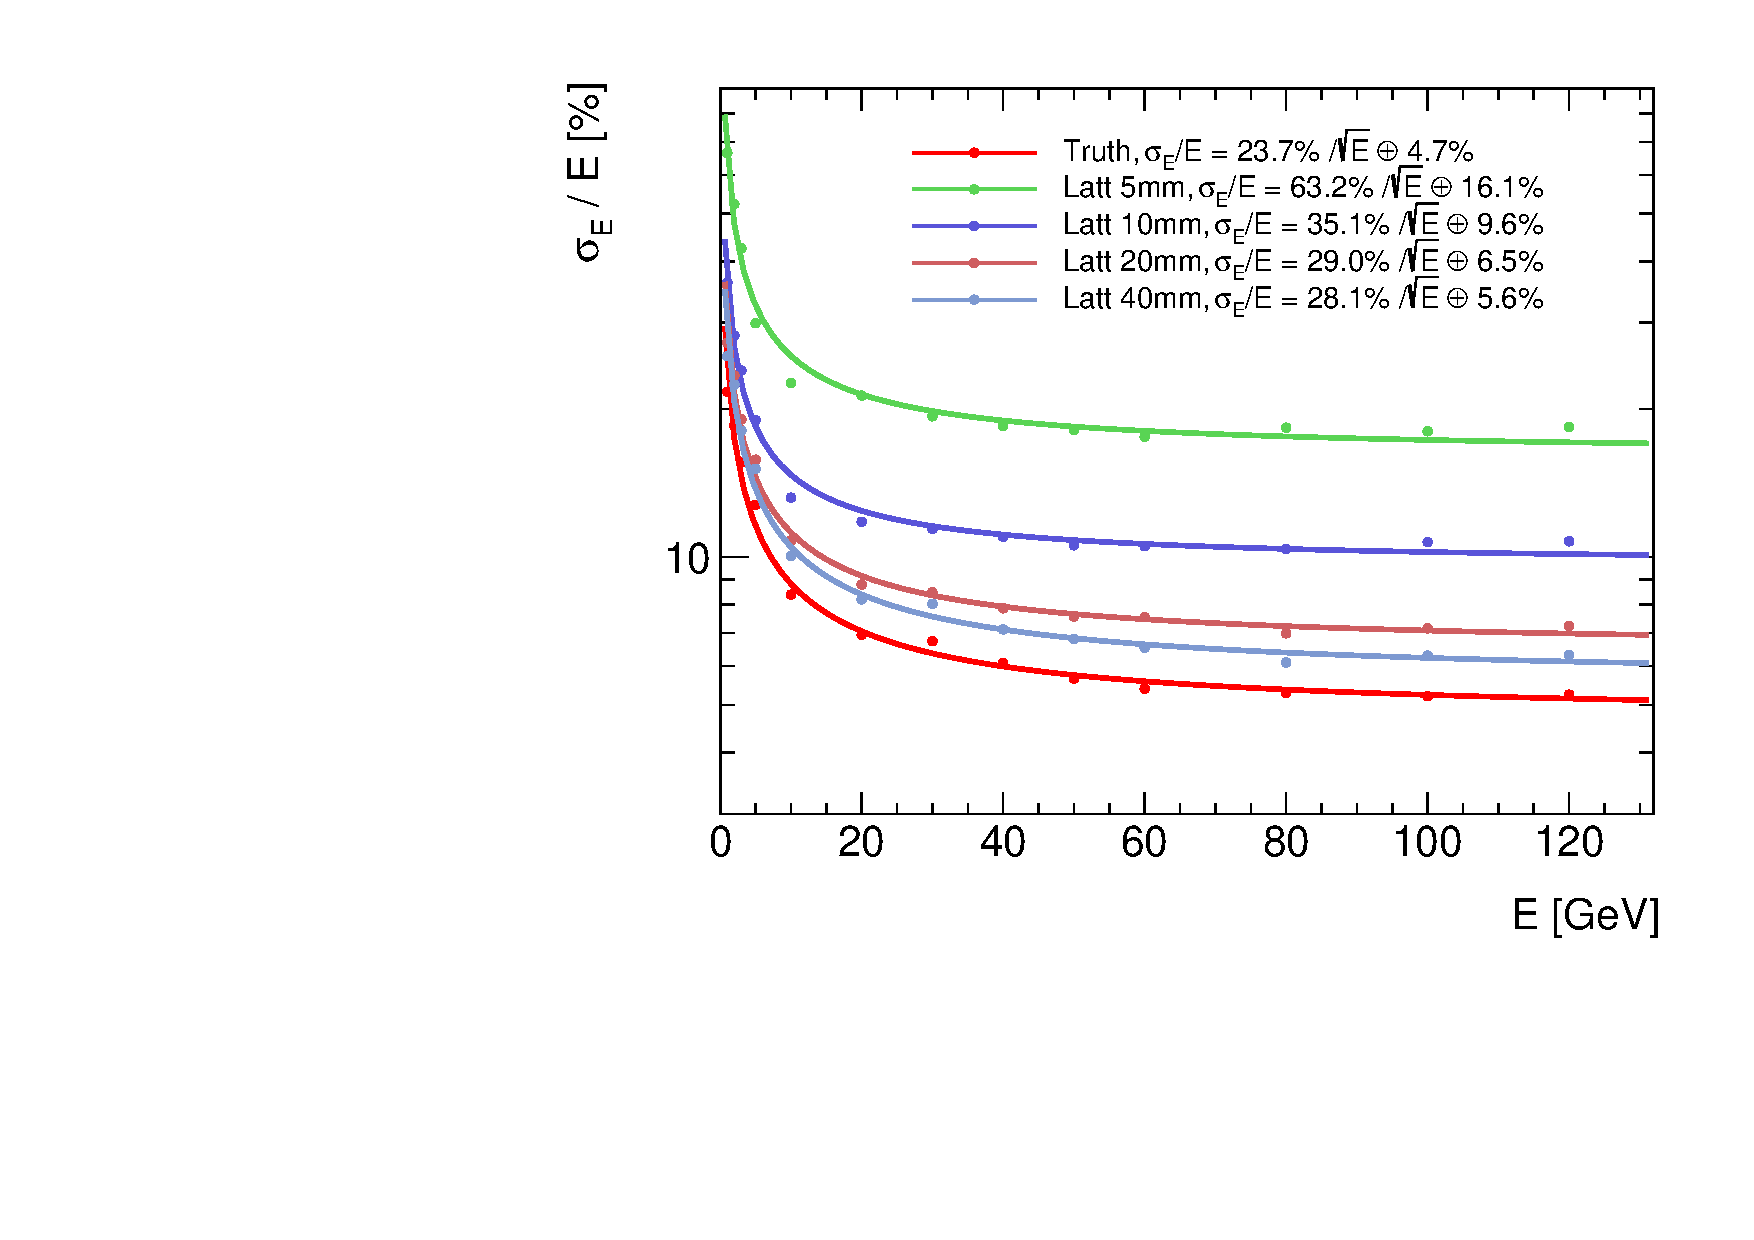
\includegraphics[width=\linewidth]{Eres_Latt_log.pdf}
  \caption{}
\end{subfigure}

\vspace{0.3cm}

\begin{subfigure}{0.48\linewidth}
  \centering
  \includegraphics[width=\linewidth]{ERes_Birks.pdf}
  \caption{}
\end{subfigure}
\caption{Simulated energy resolution as a function of
(a)~light output and readout threshold,
(b)~GS attenuation length, and
(c)~Birks' constant.}
\label{fig:Eres_vs_parameters}
\end{figure}

To confirm that longitudinal leakage dominates the constant term, the
GS-HCAL depth was increased from 48~layers ($6\,\lambdaI$) to
80~layers ($10\,\lambdaI$); the constant term dropped from 4.7\% to
2.9\% (Figure~\ref{fig:depth}).
With the full detector the ECAL (${\approx}1.2\,\lambdaI$) causes
approximately 70\% of hadrons to initiate showers upstream, which is
expected to reduce leakage significantly.
Requiring the first hadronic interaction to occur within the first two
GS-HCAL layers ($0.25\,\lambdaI$) already reduces the constant term to
approximately 3\%, consistent with PS-HCAL prototype
measurements~\cite{CALICE:2010fpb,Liu:2025hgf}.

\begin{figure}[htbp]
\centering
\begin{subfigure}{0.48\textwidth}
  \centering
  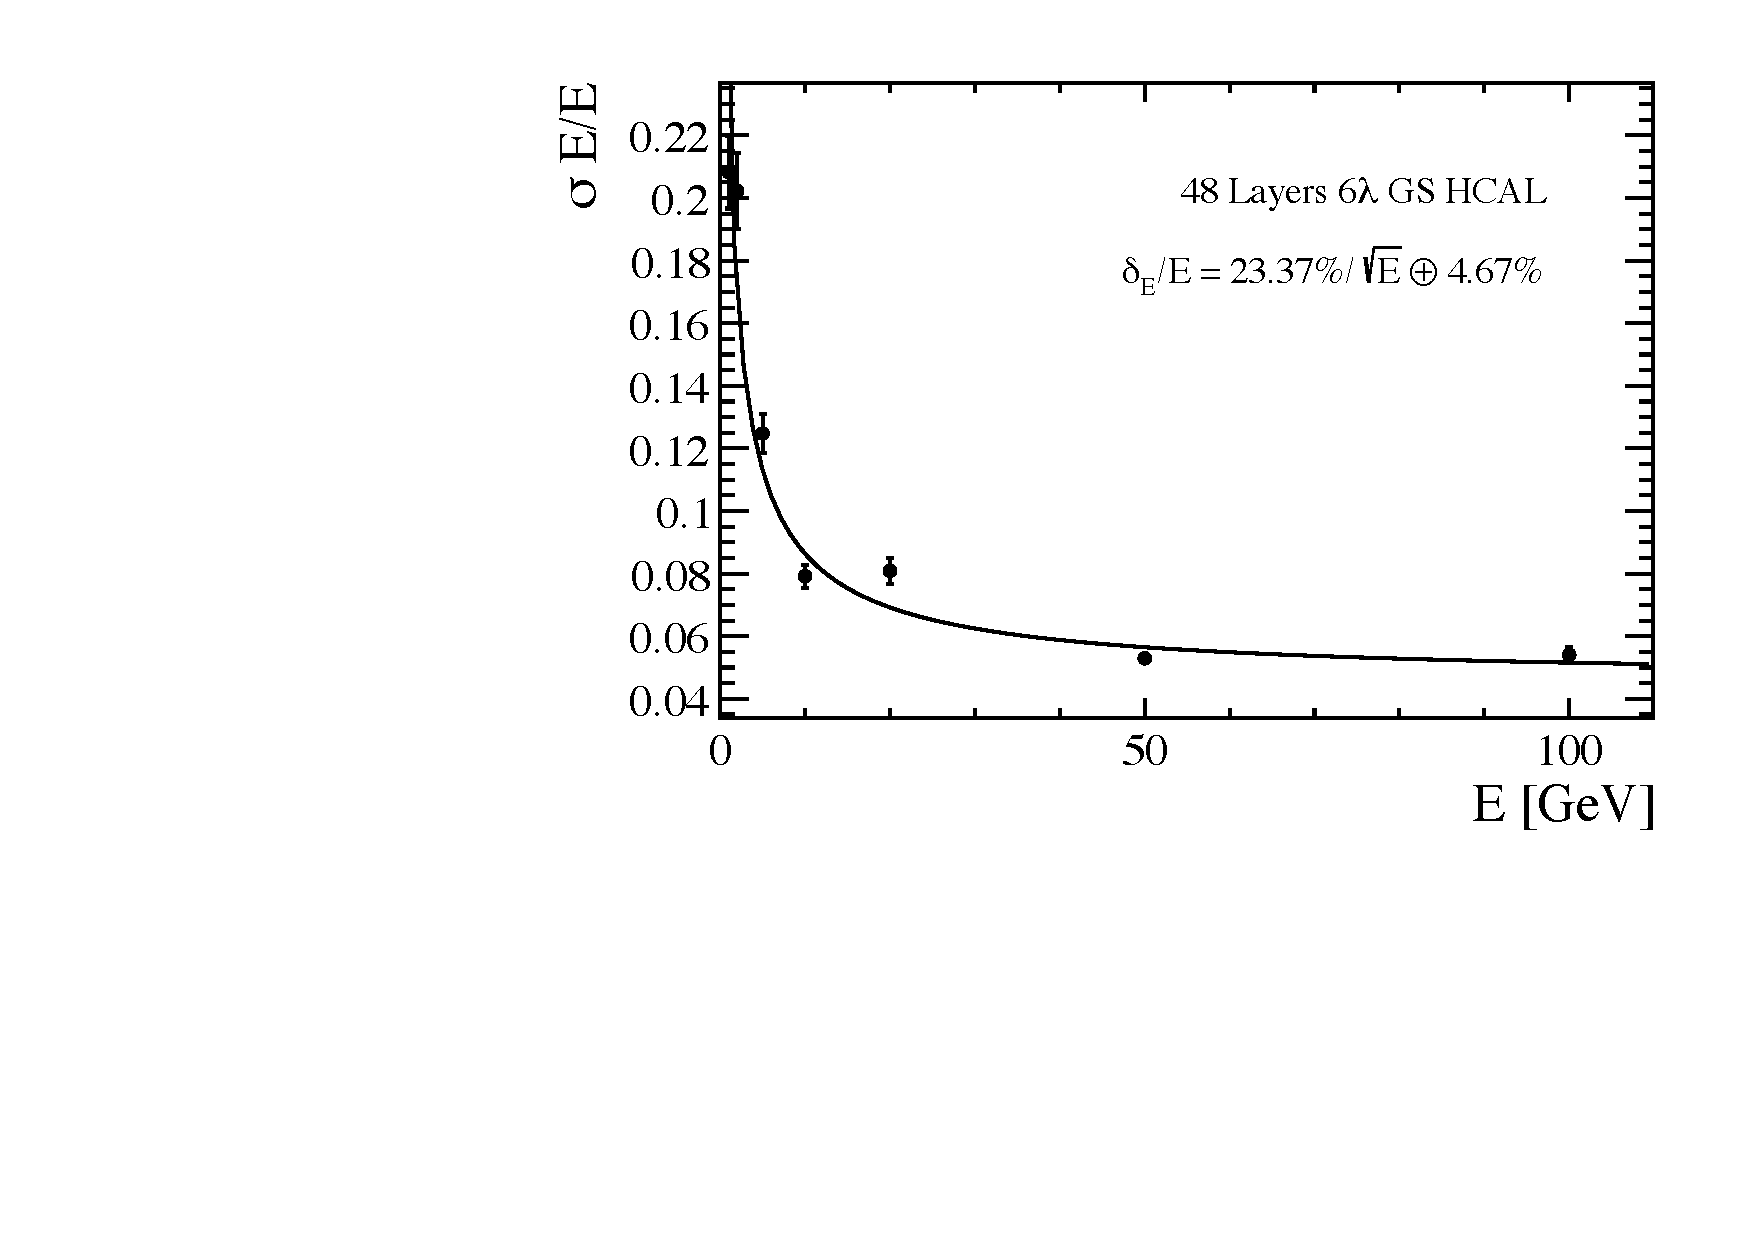
\includegraphics[width=\linewidth]{const_gs_6lambda.pdf}
  \caption{}
\end{subfigure}\hfill
\begin{subfigure}{0.48\textwidth}
  \centering
  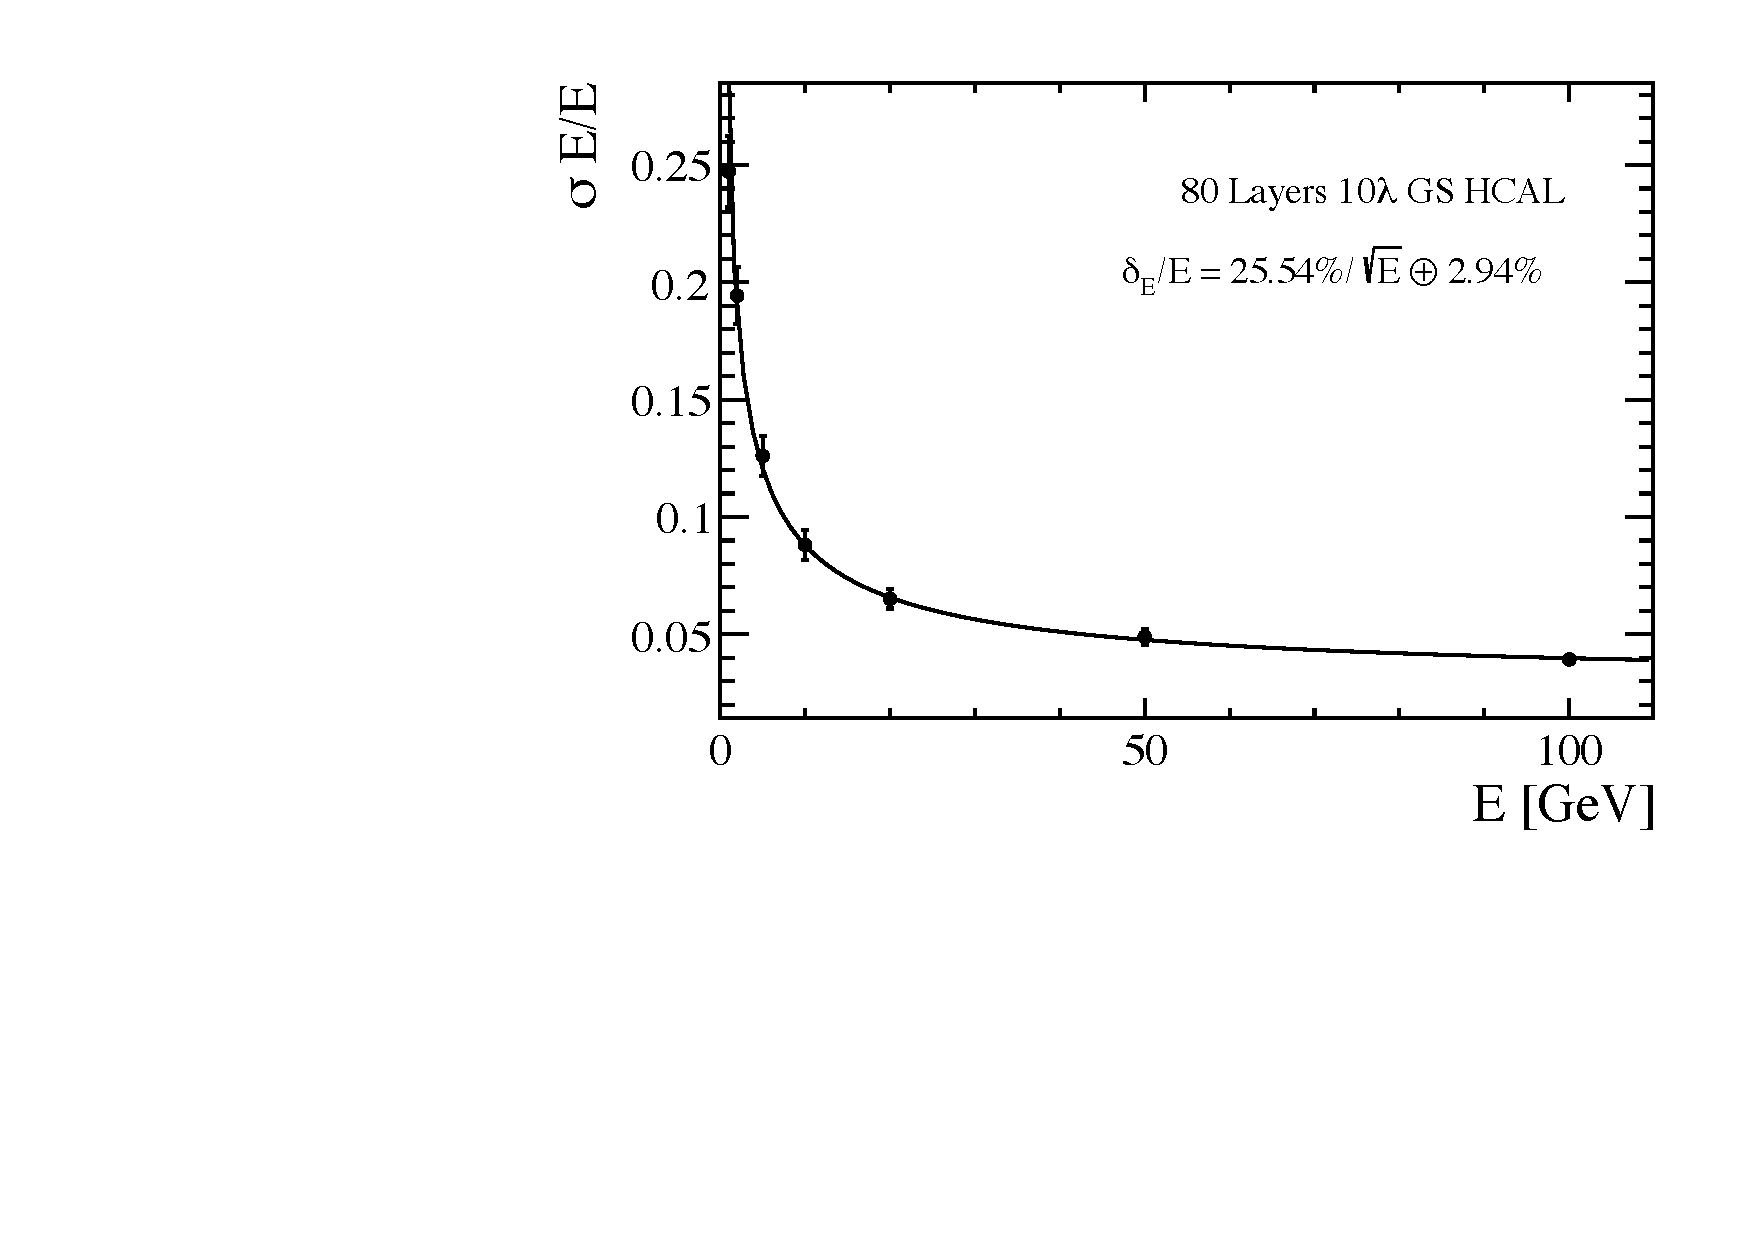
\includegraphics[width=\linewidth]{const_gs_10lambda.pdf}
  \caption{}
\end{subfigure}
\caption{Comparison of energy-resolution distributions for two GS-HCAL
depths:
(a)~$6\,\lambdaI$ (48~layers), showing a pronounced high-energy tail;
(b)~$10\,\lambdaI$ (80~layers), with the constant term reduced from
4.7\% to 2.9\%.}
\label{fig:depth}
\end{figure}

%% --------------------------------------------------------------------
\subsection{Electron--hadron response}
\label{subsec:eresponse}
%% --------------------------------------------------------------------

The calorimeter response to electrons and various hadrons was studied
using full Geant4 simulations of the standalone GS-HCAL (no upstream
ECAL).
The true energy $E_{\mathrm{true}}$ is fitted against the raw
calorimeter signal $S_{\mathrm{HCAL}}$ using a linear model
$E_{\mathrm{true}}=C\times S_{\mathrm{HCAL}}$, extracting a calibration
constant $C$ for each particle species.
The ratio $C_{\mathrm{hadron}}/C_{e}$, summarised in
Table~\ref{tab:eoverh_hcal}, quantifies the degree of non-compensation:
a value exceeding unity indicates that the hadron of a given energy
produces a smaller signal than an electron of the same energy.
The measured ratios of 1.09--1.14 are consistent with expectations for a
non-compensating sampling calorimeter~\cite{Akchurin:2012zz}.

It is important to note that $C_{\mathrm{hadron}}/C_{e}$, as an
empirically measured calibration ratio, is distinct from the intrinsic
compensation ratio $e/h$ defined in the context of hadronic shower
physics.
The intrinsic $e/h$ is the true figure of merit: a value of unity
signifies perfect compensation and eliminates the degrading effect of
fluctuations in the electromagnetic shower fraction $f_{\mathrm{em}}$
on the energy resolution~\cite{Akchurin:2012zz}.
Future work will extract the $e/h$ value through detailed Geant4
simulations that separate the electromagnetic and hadronic
components of hadronic showers.
By analysing the origin of energy deposits, the average electromagnetic
fraction $\langle f_{\mathrm{em}}\rangle$ and its event-by-event
fluctuations can be determined.
A precise calibration exploiting the intrinsic $e/h$ parameter---via
software compensation or energy-weighting algorithms---is expected to
reduce the constant term in the energy resolution below 3\%.

\begin{table}[htbp]
\centering
\caption{Calibration slopes $C$ and electron--hadron response ratios
$C_{\mathrm{hadron}}/C_{e}$ for the GS-HCAL\@.}
\label{tab:eoverh_hcal}
\begin{tabular}{lcc}
\toprule
Particle & $C$ (slope) & $C_{\mathrm{hadron}}/C_{e}$ \\
\midrule
Electron  & $2.94\pm0.01$ & ---            \\
$\pi^{-}$ & $3.20\pm0.05$ & $1.09\pm0.02$ \\
$K^{+}$   & $3.28\pm0.05$ & $1.12\pm0.02$ \\
Neutron   & $3.35\pm0.07$ & $1.14\pm0.02$ \\
Proton    & $3.36\pm0.07$ & $1.14\pm0.02$ \\
\bottomrule
\end{tabular}
\end{table}

%% --------------------------------------------------------------------
\subsection{Physics performance: Higgs-boson mass resolution}
\label{subsec:physperf}
%% --------------------------------------------------------------------

The detector-level physics performance is evaluated through PFA
reconstruction of the benchmark process $H\to gg$.
Event generation uses \textsc{Whizard}\,v1.9.5~\cite{Kilian:2007gr,
Moretti:2001zz} with next-to-leading-order matrix elements; the
full detector response is modelled with Geant4\,v11.2 within the
CEPCSW framework.
Figure~\ref{fig:ch08_BMR} shows the reconstructed dijet invariant mass.
The fitted Higgs-boson mass is $126.32\pm0.04$~GeV/$c^{2}$ with
$\sigma(m_{jj})=4.90\pm0.04$~GeV/$c^{2}$, corresponding to a
boson mass resolution (BMR) of \textbf{3.88\%}, satisfying the CEPC
target of 3--4\%.

\begin{figure}[htbp]
\centering
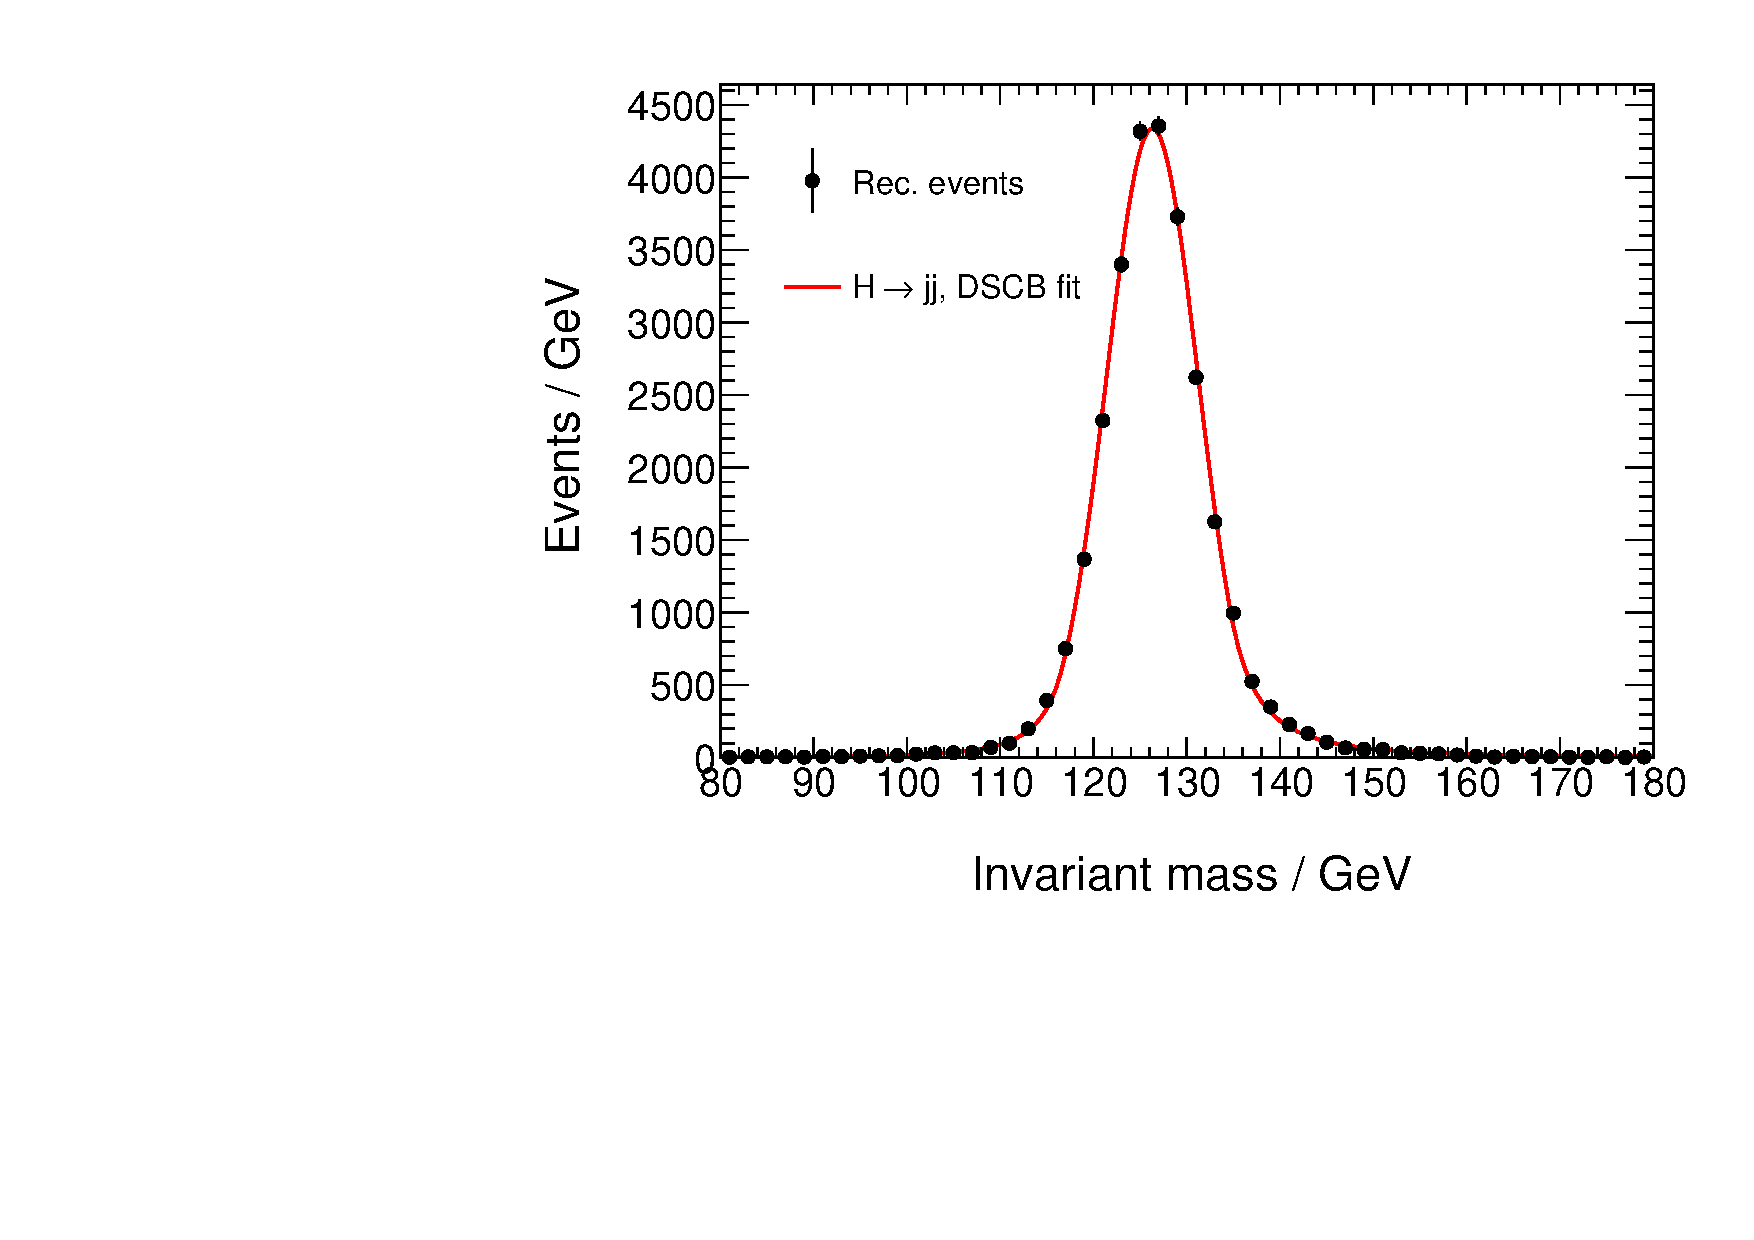
\includegraphics[width=0.60\linewidth]{Fig8.9_BMR.pdf}
\caption{Reconstructed dijet invariant mass for $H\to gg$.
Fitted mass: $126.32\pm0.04$~GeV/$c^{2}$;
$\sigma(m_{jj})=4.90\pm0.04$~GeV/$c^{2}$; BMR~=~3.88\%.}
\label{fig:ch08_BMR}
\end{figure}

%% ====================================================================
\section{Alternative HCAL technologies}
\label{sec:alternatives}
%% ====================================================================

Extensive R\&D within the CALICE Collaboration has produced well-validated
alternative technologies for PFA-based hadronic
calorimetry~\cite{CALICE:2010fpb,Baulieu:2015pfa,Bressler:2019uyt}.
These include the Digital HCAL (DHCAL)~\cite{Drake:2005eb,Bilki:2021lpo}
and Semi-Digital HCAL
(SDHCAL)~\cite{Baulieu:2015pfa,Bressler:2019uyt} using gaseous
detectors, as well as the Analog HCAL (AHCAL) based on plastic
scintillator tiles~\cite{CALICE:2010fpb}.
The dual-readout concept~\cite{Lee:2017shn,Antonello:2018sna,
Giagu:2022gmq,INFNRD-FA:2020fiu,Albergo:2025exx} has also been
investigated, though the CEPC baseline remains firmly within the PFA
paradigm.
The two most advanced PFA-compatible alternatives are summarised below.

%% --------------------------------------------------------------------
\subsection{RPC-based Semi-Digital HCAL}
\label{subsec:sdhcal}
%% --------------------------------------------------------------------

The SDHCAL~\cite{Baulieu:2015pfa,CALICE:2016fbz} employs glass
resistive-plate chambers (GRPCs) with $1\times1$~cm$^{2}$ pick-up pads
and HARDROC2 ASICs~\cite{Dulucq:2010ssa} providing 2-bit semi-digital
readout.
The prototype consists of 48~active layers inserted into a
self-supporting structure of 49 stainless-steel plates
(\SI{15}{mm} each), totalling ${\approx}6\,\lambdaI$.
Multi-threshold readout mitigates saturation effects at energies above
${\sim}\SI{30}{GeV}$~\cite{CALICE:2016fbz}.

Beam tests at CERN PS and SPS with $\pi^{-}$ beams from 3 to
\SI{80}{GeV}~\cite{CALICE:2016fbz,CALICE:2022atz} yield an energy
linearity within ${\approx}4\%$ and a resolution of
$65\%/\sqrt{E}\oplus2.5\%$ (Figure~\ref{fig:SDHCAL-Lin-Res}).

\begin{figure}[htbp]
\centering
\begin{subfigure}{0.30\linewidth}
  \centering
  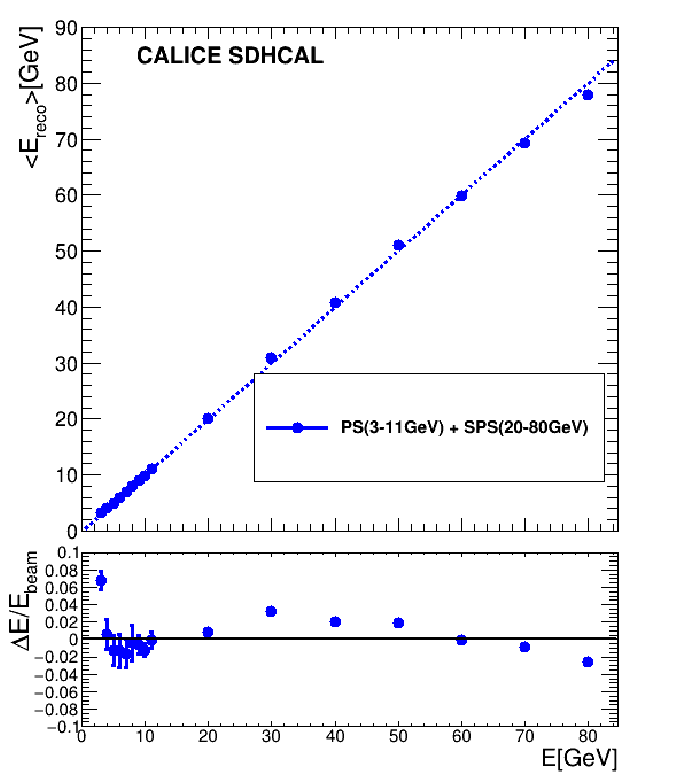
\includegraphics[width=\linewidth]{SDHCAL-Linearity-PS-SPS.pdf}
  \caption{}
\end{subfigure}\hfill
\begin{subfigure}{0.40\linewidth}
  \centering
  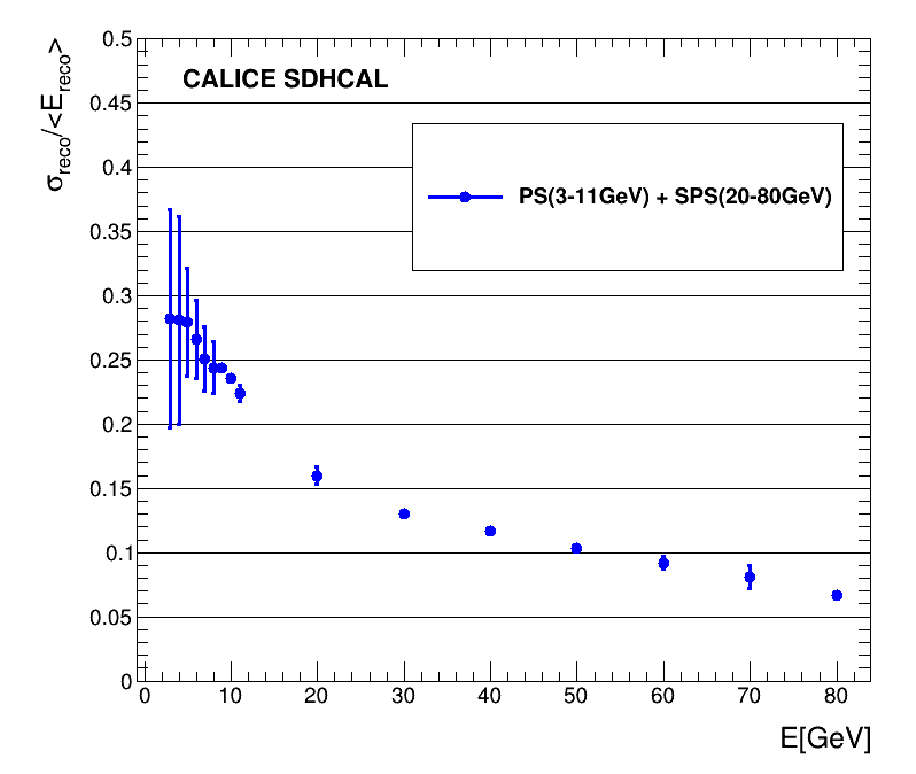
\includegraphics[width=\linewidth]{SDHCAL-Resolution-PS-SPS.pdf}
  \caption{}
\end{subfigure}
\caption{SDHCAL prototype beam-test results~\cite{CALICE:2022atz}:
(a)~energy linearity; (b)~energy resolution.}
\label{fig:SDHCAL-Lin-Res}
\end{figure}

%% --------------------------------------------------------------------
\subsection{Plastic-scintillator Analog HCAL}
\label{subsec:ahcal}
%% --------------------------------------------------------------------

The AHCAL~\cite{CALICE:2010fpb,Shi:2022fsb,Liu:2025hgf} uses
injection-moulded plastic-scintillator tiles
($40\times40\times\SI{10}{mm^{3}}$, later \SI{3.5}{mm} thick) wrapped
in ESR film and read out by SiPMs.
It was the baseline HCAL design in the CEPC Conceptual Design Report
(CDR), and remains a mature and well-validated fallback technology.
Extensive simulation studies have addressed optimal absorber
thickness, sampling-layer count, and cell size~\cite{Shi:2022fsb,Liu:2025hgf}.
A technological prototype of $72\times72\times\SI{120}{cm^{3}}$
(40~layers, $4.7\,\lambdaI$, 12\,960 channels) was developed by USTC,
SJTU, and IHEP, and tested at CERN SPS and PS\@.
Approximately 15\,000 plastic tiles were characterised with a $^{90}$Sr
source, yielding a mean light output of ${\approx}12.9$~\peMIP with
91.6\% of tiles within a 10\% uniformity window~\cite{Duan:2021mvk}.

The readout uses SPIROC2E
ASICs~\cite{Bouchel:2011zz,ConfortiDiLorenzo:2013vka,Callier:2009uoa}
with 36~channels each and dual-gain preamplifiers.
Three beam-test campaigns at CERN collected approximately 65~million
events, and advanced machine-learning methods were applied for particle
identification~\cite{Song:2023ceh}.
The measured energy linearity is better than 1.5\% and the energy
resolution is $56.2\%/\sqrt{E}\oplus2.5\%$~\cite{Liu:2025hgf}
(Figure~\ref{fig:Figure8}).
Software-compensation algorithms exploiting the high granularity can
improve the hadronic energy resolution by up to
30\%~\cite{Israeli:2018byq,Simon:2009bt}.

\begin{figure}[htbp]
\centering
\begin{subfigure}{0.35\linewidth}
  \centering
  \includegraphics[width=\linewidth]{Fig8-a.pdf}
  \caption{}
\end{subfigure}\hfill
\begin{subfigure}{0.45\linewidth}
  \centering
  \includegraphics[width=\linewidth]{Fig8-b.pdf}
  \caption{}
\end{subfigure}
\caption{AHCAL prototype performance with high-energy $\pi^{-}$
beams~\cite{Liu:2025hgf}:
(a)~energy linearity (better than 1.5\%);
(b)~energy resolution ($56.2\%/\sqrt{E}\oplus2.5\%$, red curve).}
\label{fig:Figure8}
\end{figure}

%% ====================================================================
\section{Summary and outlook}
\label{sec:summary}
%% ====================================================================

The GS-HCAL has been presented as the baseline hadronic calorimeter for
the CEPC reference detector, employing high-density GFO
glass-scintillator cells read out by SiPMs in a barrel and two endcaps
totalling approximately 5.22~million channels.

The principal R\&D achievements reported in this paper are:
\begin{itemize}
\item Development of GFO glass with a light yield exceeding
  \SI{1000}{\phMeV}, an attenuation length of ${\approx}\SI{6}{cm}$,
  and radiation tolerance retaining more than 70\% of the initial light
  yield at \SI{100}{Gy}.
\item Single-cell measurements demonstrating $63.6\pm0.5$~\peMIP with
  cosmic muons and $157.6\pm2.9$~\peMIP with \SI{5}{GeV} electrons at
  KEK\@.
\item A custom pre-amplifier FEE with \SI{400}{MHz} bandwidth and
  $300\,\mu\mathrm{V}_\mathrm{RMS}$ noise.
\item Geant4 simulation yielding $\sigma_{E}/E =
  29.8\%/\sqrt{E}\oplus6.5\%$ and a Higgs BMR of 3.88\% for $H\to gg$.
\item A validated mechanical design with deformation below \SI{0.66}{mm}
  under assembly loads and adequate margin when supporting the
  \SI{135}{t} ECAL\@.
\end{itemize}

The constant term of ${\approx}5$--6\%, while sufficient for the
3--4\% BMR target, can be further reduced below 3\% through:
(i)~improved calibration exploiting the intrinsic $e/h$ ratio extracted
from shower-component decomposition;
(ii)~energy-weighting and software-compensation algorithms;
(iii)~position-dependent light-collection efficiency corrections; and
(iv)~machine-learning-based shower
reconstruction~\cite{Simon:2009bt,Rolph:2022eba,CALICE:2024imr,Liu:2025hgf}.

The GS-HCAL development follows a phased timeline:
\begin{itemize}
\item \textbf{2024--2025:} finalise the \cellsize tile design and begin
  mass production of ${\sim}10\,000$ prototype tiles.
\item \textbf{2026:} complete the \SI{0.6}{m^{3}} prototype (8112~tiles)
  and begin beam tests at CSNS or CERN\@.
\item \textbf{2027:} integrate a full-scale module and validate
  performance with cosmic-ray and test-beam data.
\end{itemize}

Ongoing and planned R\&D includes: further optimisation of the GS light
output and attenuation length; evaluation of emerging SiPM devices;
development of a custom low-power (\SI{15}{mW/channel}) ASIC for the
final readout system; and integration of the HCAL electronics into the
CEPC-wide data-acquisition architecture.

The SDHCAL and AHCAL alternatives, with beam-test-confirmed energy
resolutions of $65\%/\sqrt{E}\oplus2.5\%$ and
$56\%/\sqrt{E}\oplus2.5\%$, respectively, provide important benchmarks
and contingency pathways.
The results presented in this paper establish a strong foundation for
realising a high-performance, cost-effective hadronic calorimeter for the
CEPC\@.

%% ====================================================================
\section*{Acknowledgements}
%% ====================================================================

The authors thank all members of the CEPC Study Group for their
contributions to the physics and detector design studies.
We are grateful to the CALICE Collaboration for extensive test-beam data
and collaborative R\&D efforts, and to the staff of the KEK test-beam
facility and the APEP proton-irradiation facility for experimental
support.
This work is supported in part by
the National Key Research and Development Program of China
(Grant No.~2020YFA0406200),
the Chinese Academy of Sciences (Grant No.~XDB34000000),
the National Natural Science Foundation of China (NSFC,
Grant Nos.~12075265 and~12105295),
and the CEPC detector R\&D programme.
%% [PLACEHOLDER — verify grant numbers and add institution-level funding
%%  acknowledgements before submission]

%% ====================================================================
%% References
%% ====================================================================
\bibliographystyle{elsarticle-num}
\bibliography{gshcal}  %% bib file: gshcal.bib

\end{document}
